% !TEX encoding = UTF-8 Unicode

\documentclass[twoside,12pt,a4paper]{book}

% !TEX root = ../Saunkin.tex
% !TEX encoding = UTF-8 Unicode

% Macros for LateX

%\usepackage[bf,small]{caption}
\usepackage[colorlinks,linkcolor=blue,linktocpage]{hyperref} % backref pargebackref
\usepackage[fleqn]{amsmath}
\usepackage[greek,english]{babel}
\usepackage{alphabeta}
\usepackage[square,comma,sort&compress,numbers]{natbib}     %% Citation package
\usepackage[toc,page]{appendix}
% \usepackage[T1]{fontenc}
% \usepackage[utf8]{inputenc}
\usepackage{amssymb}                                %% Special AMS symbols
\usepackage{array}                                  %% Extra's for formatting tables
\usepackage{calc}
\usepackage{comment}
\usepackage{enumerate}
\usepackage{epigraph}
%\usepackage{epsfig}
\usepackage{fancyhdr}                               %% Fancy header definition
\usepackage{graphicx}
\usepackage{hhline}
\usepackage{hyperref}
\usepackage{listings}
%\usepackage{losnotations}
%\usepackage{losymbol}
\usepackage{makeidx}
\usepackage{multicol}
\usepackage{setspace}
\usepackage{subfigure}
\usepackage{url}
\usepackage{ucs}
\usepackage{babelbib}
\usepackage{float}
\usepackage{textcomp}
\usepackage[shortcuts]{extdash}
\usepackage{listings}
\usepackage{verbatim}
\usepackage{color}
\usepackage{colortbl}
\usepackage[table]{xcolor}
\usepackage[figure,vlined,linesnumbered]{algorithm2e}
\usepackage{tablefootnote}


%
% Page definitions
%
\setlength{\textheight}{23cm}
\setlength{\textwidth}{15.5cm}
\setlength{\oddsidemargin}{0.2cm}
\setlength{\evensidemargin}{0.2cm}
\setlength{\topmargin}{-0.5cm}
\setlength{\headsep}{1cm}
%\setlength{\topmargin}{-1.2cm}

\renewcommand{\baselinestretch}{1.5}

\setcounter{topnumber}{2}       % Maximum # of floats at top of page
\setcounter{bottomnumber}{2}    % Maximum # of floats at bottom of page
\setcounter{totalnumber}{3}     % Maximum total # of floats on one page
\setcounter{secnumdepth}{5}

\vfuzz1pc   % Don't bother to report overfull boxes if over-edge is < 1pc
\hfuzz1pc   % Don't bother to report overfull boxes if over-edge is < 1pc

\sloppy

\frenchspacing

%\bibliographystyle{hellas}


%
% Header
%

%  \def\ps@headings{%
%      \let\@oddfoot\@empty\let\@evenfoot\@empty
%      \def\@evenhead{\thepage\hfil\slshape\leftmark}%
%      \def\@oddhead{{\slshape\rightmark}\hfil\thepage}%
%      \let\@mkboth\markboth
%    \def\chaptermark##1{%
%      \markboth {\textsc{ %\MakeUppercase{% hack it......
%        \ifnum \c@secnumdepth >\m@ne
%          \if@mainmatter
%            \@chapapp\ \thechapter. \ %
%          \fi
%        \fi
%        ##1}}{}}%
%    \def\sectionmark##1{%
%      \markright {\textsc{ %\MakeUppercase{% hack it......
%        \ifnum \c@secnumdepth >\z@
%          \thesection. \ %
%        \fi
%        ##1}}}}

%\renewcommand{\chaptermark}[1]{\if@mainmatter
%                                \markboth{Κεφάλαιο \thechapter}{} \markright{#1}
%                               \else
%                                \markboth{#1}{#1}
%                               \fi}
%\renewcommand{\sectionmark}[1]{\markright{\thesection\ #1}}
%
%

%\pagestyle{fancy}
%\fancyhf{}
\fancyhead[RO]{\textsc{\footnotesize\rightmark}}
\fancyhead[LE]{\textsc{\footnotesize\leftmark}}
\fancyhead[RE,LO]{}
\fancyfoot[CE,CO]{}
\fancyfoot[LE,RO]{\thepage}


% Command \SetFigFont does NOTHING !!!!!!
\newcommand{\SetFigFont}[3]{}

%
% Languages
%
\newcommand{\eng}{\selectlanguage{english}}
\newcommand{\gre}{\selectlanguage{greek}}
\def\slg{ \selectlanguage{greek} }
\def\sla{ \selectlanguage{american} }


% Code

\makeatletter
\newenvironment{vercode}{%
\latintext\par
\def\verbatim@processline{\the\verbatim@line\\ }%
\def\@verbatim{\the\every@verbatim
  \obeylines
  \let\do\@makeother \dospecials
  \verbatim@font
}%
\def\endverbatim{\endgroup}%
\noindent
\verbatim}{\endverbatim}
\makeatother

\definecolor{lightgray}{gray}{0.9}
\definecolor{codegreen}{rgb}{0,0.6,0}
\definecolor{codegray}{rgb}{0.5,0.5,0.5}
\definecolor{codepurple}{rgb}{0.58,0,0.82}
\definecolor{backcolour}{rgb}{0.95,0.95,0.92}
 
\lstdefinestyle{mystyle}{
    backgroundcolor=\color{backcolour},   
    commentstyle=\color{codegreen},
    keywordstyle=\color{magenta},
    numberstyle=\tiny\color{codegray},
    stringstyle=\color{codepurple},
    basicstyle=\footnotesize,
    breakatwhitespace=false,         
    breaklines=true,                 
    captionpos=b,                    
    keepspaces=true,                 
    numbers=left,                    
    numbersep=5pt,                  
    showspaces=false,                
    showstringspaces=false,
    showtabs=false,                  
    tabsize=2,
    columns=flexible,
    literate=%
{α}{{\textgreek{a}}}1%
{ά}{{\textgreek{'a}}}1%
{β}{{\textgreek{b}}}1%
{γ}{{\textgreek{g}}}1%
{δ}{{\textgreek{d}}}1%
{ε}{{\textgreek{e}}}1%
{έ}{{\textgreek{'e}}}1%
{ζ}{{\textgreek{z}}}1%
{η}{{\textgreek{h}}}1%
{ή}{{\textgreek{'h}}}1%
{θ}{{\textgreek{j}}}1%
{ι}{{\textgreek{i}}}1%
{ί}{{\textgreek{'i}}}1%
{ϊ}{{\textgreek{"i}}}1%
{ΐ}{{\textgreek{'"i}}}1%
{κ}{{\textgreek{k}}}1%
{λ}{{\textgreek{l}}}1%
{μ}{{\textgreek{m}}}1%
{ν}{{\textgreek{n}}}1%
{ξ}{{\textgreek{x}}}1%
{ο}{{\textgreek{o}}}1%
{ό}{{\textgreek{'o}}}1%
{π}{{\textgreek{p}}}1%
{ρ}{{\textgreek{r}}}1%
{σ}{{\textgreek{sv}}}1%
{ς}{{\textgreek{c}}}1%
{τ}{{\textgreek{t}}}1%
{υ}{{\textgreek{u}}}1%
{ύ}{{\textgreek{'u}}}1%
{ϋ}{{\textgreek{"u}}}1%
{ΰ}{{\textgreek{'"u}}}1%
{φ}{{\textgreek{f}}}1%
{χ}{{\textgreek{q}}}1%
{ψ}{{\textgreek{y}}}1%
{ω}{{\textgreek{w}}}1%
{ώ}{{\textgreek{'w}}}1%
{Α}{{\textgreek{A}}}1%
{Β}{{\textgreek{B}}}1%
{Γ}{{\textgreek{G}}}1%
{Δ}{{\textgreek{D}}}1%
{Ε}{{\textgreek{E}}}1%
{Ζ}{{\textgreek{Z}}}1%
{Η}{{\textgreek{H}}}1%
{Θ}{{\textgreek{J}}}1%
{Ι}{{\textgreek{I}}}1%
{Κ}{{\textgreek{K}}}1%
{Λ}{{\textgreek{L}}}1%
{Μ}{{\textgreek{M}}}1%
{Ν}{{\textgreek{N}}}1%
{Ξ}{{\textgreek{X}}}1%
{Ο}{{\textgreek{O}}}1%
{Π}{{\textgreek{P}}}1%
{Ρ}{{\textgreek{R}}}1%
{Σ}{{\textgreek{S}}}1%
{Τ}{{\textgreek{T}}}1%
{Υ}{{\textgreek{U}}}1%
{Φ}{{\textgreek{F}}}1%
{Χ}{{\textgreek{Q}}}1%
{Ψ}{{\textgreek{Y}}}1%
{Ω}{{\textgreek{W}}}1%
{À}{{\`{A}}}1%
{È}{{\`{E}}}1%
{É}{{\'{E}}}1%
{Ì}{{\`{I}}}1%
{Ò}{{\`{O}}}1%
{à}{{\`{a}}}1%
{è}{{\`{e}}}1%
{é}{{\'{e}}}1%
{ì}{{\`{i}}}1%
{ò}{{\`{o}}}1%
{ù}{{\`{u}}}1%
}

\lstset{style=mystyle}


%
\SetKwInOut{Input}{Input}
\SetKwInOut{Output}{Output}
\SetKwInput{Algorithm}{Algorithm}
\SetKwInput{Remark}{Remark}
\SetKw{Let}{Let}
\SetKw{while}{while}
\SetKw{Add}{Add}
\SetKwFor{While}{while}{do}{endw}
\SetKwComment{Comment}{{// }}{}


% Math
\newtheorem{definition}{Definition}
\newtheorem{proposition}{Proposition}[section]
\newtheorem{theorem}{Theorem}[section]
\newtheorem{corollary}{Corollary}[section]
\newtheorem{lemma}{Lemma}[section]
\newtheorem{example}{Example}
\newtheorem{remark}{Remark}[section]
\newtheorem{notation}{Notation}[section]

\newcommand{\proof}{\noindent {\bf Proof:\ }}
\newcommand{\defEnd}{\ \rule[-0.25mm]{0.25cm}{0.25cm}}
\renewenvironment{proof}{\noindent\textbf{Proof:}}{\rule[-0.25mm]{0.25cm}{0.25cm}\vspace{1.8ex}}

%\newenvironment{proof}{{\bf Proof:}}{\rule[-0.25mm]{0.25cm}{0.25cm}}
%\newcommand{\proofEnd}{\ \rule[-0.25mm]{0.25cm}{0.25cm}}
%\newenvironment{remark}{{\bf Remark:}}{\rule[-0.25mm]{0.25cm}{0.25cm}}

%\newcommand{\proof}{\noindent {\bf Proof:\ }}

%\newcommand{\defEnd}{\ \rule[-0.25mm]{0.25cm}{0.25cm}}
%\newcommand{\smalltb}{\hspace*{.5cm}}

% logical connectives
%\newcommand{\And}{\land}
\newcommand{\Or}{\lor}
\newcommand{\Then}{\Longrightarrow}
%\newcommand{\If}{\longleftarrow}
\newcommand{\then}{\Longrightarrow}
%\newcommand{\implies}{\supset}
\newcommand{\Equiv}{\equiv}
\newcommand{\Iff}{\Longleftrightarrow}
% do not add \; to \bigAnd and \bigOr
\newcommand{\bigAnd}{\bigwedge}
\newcommand{\bigOr}{\bigvee}
\newcommand{\poss}{\raisebox{-.2ex}{$\Diamond$}}
\newcommand{\nec}{\raisebox{-.2ex}{$\Box$}}
\newcommand{\cert}{\raisebox{-.2ex}{$\Box$}}
\newcommand{\blackcirc}{\mbox{$\bigcirc \hspace*{-.75em} \bullet \ $}}
\newcommand{\contains}{\sqsupset}

% set operations
%\newcommand{\complement}[1]{\overline{#1}}
\newcommand{\union}{\cup}
\newcommand{\bigunion}{\bigcup}
\newcommand{\bigUnion}{\bigcup}
\newcommand{\intersection}{\cap}
\newcommand{\bigintersection}{\bigcap}
\newcommand{\bigIntersection}{\bigcap}
\newcommand{\maps}{\;\longrightarrow\;}

% qq for "quine's quotes
\newcommand{\lqq}{\mathopen{\raisebox{-.5ex}{${}^{{}^\lceil}$}\mskip-2.5mu}}
\newcommand{\rqq}{\mathclose{\raisebox{-.5ex}{${}^{{}^\rceil}$}}}
\newcommand{\qq}[1]{\lqq{#1}\rqq}

% others
%\newcommand{\bar}[1]{\overline{#1}}
\newcommand{\tld}[1]{\widetilde{#1}}   % wide tilde
\newcommand{\wht}[1]{\widehat{#1}}      % wide hat
\newcommand{\tb}{\hspace*{0.25in}}
%\newcommand{\tb}{\hspace*{3ex}}
\newcommand{\htb}{\hspace*{0.12in}}
\newcommand{\xor}{\,\otimes\,}
%\newcommand{\comment}[1]{}
\newcommand{\pair}[2]{\langle#1,#2\rangle}
\newcommand{\throu}[2]{#1\ (D\; E\; S\; F)\ #2}
\newcommand{\comb}[2]{\left( \begin{array}{c} #1 \\ #2 \end{array} \right)}
\newcommand{\abs}[1]{\left|#1\right|}
\newcommand{\size}[1]{\left\|#1\right\|}
%\newcommand{\Intg}{{\Bbb Z}}
\newcommand{\Rat}{{\Bbb Q}}
\newcommand{\Real}{{\Bbb R}}

\newcommand{\N}{{\Bbb N}}
%\newcommand{\Intg}{{\cal Z}}
%\newcommand{\Rat}{{\cal Q}}
%\newcommand{\Real}{{\cal R}}

\newcommand{\Int}{{\sf I}}   % intervals
\newcommand{\tmodels}{\models_{\cal T}}
\newcommand{\proves}{\vdash}
\newcommand{\kf}[1]{\underline{\sf {#1}}}
\newcommand{\mytheta}{\;\theta\;}
\newcommand{\myxi}{\;\xi\;}
%\newcommand{\m}[1]{$\sf {#1}$}
\newcommand{\clog}[1]{\[\sf {#1} \]}
\newcommand{\arr}{$\rightarrow$}
%\newcommand{\inft}{$\infty$}
\newcommand{\la}{$\langle$}
\newcommand{\ra}{$\rangle$}
\newcommand{\ch}{$\ $}
\newcommand{\join}{\Join}

\newcommand{\In}{\;in\;}
\newcommand{\Isa}{\;isA\;}
\newcommand{\isA}{\;isA\;}

% thesis macros
% languages
\newcommand{\con}{{\cal C}}
\newcommand{\lang}{{\cal L}}
\newcommand{\langp}{{\cal L}^+}

% the structures of the above languages
\newcommand{\Mlang}{{\bf M}_{\cal L}}
\newcommand{\Mlangp}{{\bf M}_{{\cal L}^+}}

% languages
%\newcommand{\diPCL}{{\rm diPCL}}
%\newcommand{\diTCL}{{\em diTCL}}
%\newcommand{\dePCL}{{\em dePCL}}
%\newcommand{\deTCL}{{\em deTCL}}

% structures for the above languages
\newcommand{\Sd}{{\bf D}}
\newcommand{\Sz}{{\bf Z}}
\newcommand{\Sq}{{\bf Q}}

\newcommand{\Szi}{{\bf ZI_Z}}
\newcommand{\Sqi}{{\bf QI_Q}}

\newcommand{\Sdz}{{\bf DZ}}
\newcommand{\Sdq}{{\bf DQ}}

\newcommand{\Sdzi}{{\bf DZI_Z}}
\newcommand{\Sdqi}{{\bf DQI_Q}}


% Chronos reports
\newcommand{\val}{\rightarrow}

\def\ibi{\textbf{\textit{i}}}
\def\ibj{\textbf{\textit{j}}}

% Anomalies
%\def\rem#1{\marginpar{\scriptsize #1}}
\def\rem#1{}
\def\nnn{~\\-------\\}

\def\np{\ensuremath{\cal NP}}
\def\oo{{\cal O}}
\def\ibi{\textbf{\textit{i}}}
\def\ibj{\textbf{\textit{j}}}
\def\fand{\mbox{  and  }}
\def\sup{\mathit{sup}}
\def\inf{\mathit{inf}}
\def\lv{\mbox{``}}
\def\rv{\mbox{"}}
\def\size#1{|\:#1\:|}
%\def\restr#1#2{\mathit{Restrict}(#1,#2)}
%\def\st#1{\mathit{Subtext}(#1)}
\def\ep#1{\mathit{Epoints}(#1)}
\def\wo#1{\mathit{Words}(#1)}

% Cheats
\def\figspa{\vspace{-1ex}}
\def\figspb{\vspace{-3ex}}
\def\figspc{\vspace{-4ex}}


\newcommand{\attn}[1]{ {\bf {[*** #1 ***]}}}

% Titles
\newcommand{\stitle}[1]{\vspace{.5ex}\noindent\textbf{#1}}
\newcommand{\sititle}[1]{\vspace{.2ex}\noindent\textit{#1}}
\newcommand{\sstitle}[1]{\vspace{.5ex}\noindent\textbf{#1}}

% Lists
\newenvironment{mylisting}[1] {\vspace*{-1ex} \begin{list}{$\bullet$}{
	\usecounter{enumi}
	\setlength{\labelwidth}{2ex}
	\setlength{\labelsep}{1ex}
	\setlength{\leftmargin}{2.5ex}
	\setlength{\rightmargin}{0ex}
	\setlength{\itemsep}{0.4ex}
	\setlength{\parsep}{0ex}
} #1 } {\end{list}}


\def\rem#1{\marginpar{\scriptsize #1}}
\newcommand{\snote}[1]{\textbf{\textcolor{teal}{#1}}}
\newcommand{\enote}[1]{\textbf{\textcolor{blue}{#1}}}
\newcommand{\scor}[2]{\textbf{\textcolor{red}{#1}} $\rightarrow$ \textbf{\textcolor{teal}{#2}}}
\def\nnn{~\\-------\\}
%\def\rem#1{\marginpar{\scriptsize{\textcolor{green}{#1}}}}
%\def\rem#1{{\scriptsize{\textcolor{green}{#1}}}}
\def\rem#1{}


\newcommand{\commentg}[1]{\noindent
\colorbox{lightgray}{\parbox{\textwidth}{%
 \vskip5pt
 \leftskip5pt\rightskip5pt
 #1
 \vskip5pt
 }
}
}

\rowcolors{1}{}{lightgray}

% % !TEX encoding = UTF-8 Unicode
% !TEX root = ../Saunkin.tex

% \selectlanguage{english}
% \hyphenation{
% data-base data-bases
% net-works lan-gu-a-ges
% and ETL for Graphs provider TMR
% }

%\selectlanguage{greek}
%\hyphenation{
%ατό-μι-κης αρι-θμούς αντι-κει-μέ-νων απα-λοι-φής απρό-σκο-πτης αλγό-ριθ-μοι
%αλγό-ριθ-μος απο-τε-λέ-σμα-τα ανα-ζη-τη-θούν αυ-τής αντι-κα-τα-στά-σεις
%αντι-κει-με-νο-στρε-φείς αυθ-ύπ-αρ-κτη ανα-πα-ρά-στα-ση αρχι-τε-κτο-νι-κής
%ανα-πα-ρά-στα-ση
%%
%βι-βλιο-γρα-φία
%%
%για γραμ-μές γραμ-μι-κών γνω-στι-κό
%%
%δου-λέ-ψω δύο δί-σκους δε-δο-μέ-νων δε-δο-μέ-να διεπα-φές δεικτοδότησης
%δέν-τρου δια-πι-στώ-νε-ται Δι-κτύων Δια-χεί-ρι-σης δια-χεί-ρι-σης
%%
%εθνι-κό επο-μέ-νως επαρ-κούν εμπει-ρία επι-πρό-σθε-τα επι-κεντρώ-θη-κε έρευ-να
%Ευρω-παϊ-κής εξα-γω-γής ερω-τή-σεων έρευ-νά έρευ-να
%%
%ηλεκ-τρο-λό-γων ημε-ρο-μη-νίες
%%
%κα-τεύ-θυν-σης κλά-σης κλά-σεις κύ-βων
%%
%λο-γι-κής
%%
%μέ-θο-δος μο-ντέ-λο μο-ντέ-λα με-τα-βλη-τές
%%
%οντο-τήτων
%%
%Στην συ-γκε-κρι-με-νο-ποιού-νται συ-στη-μά-των συν-αθροι-στι-κή σχε-δία-ση
%σχη-μα-τί-ζο-νται συ-γκρού-σεων
%%
%Τεχνη-τής Νοη-μο-σύ-νης τμή-μα τυ-χαί-ους τις την Τη-λε-πι-κοι-νω-νιών
%%
%ορί-στη-κε Ομοίως όπως ορι-σμέ-νους ορι-σμούς ορι-σμοί ολο-κλη-ρώ-σου-με
%%
%πα-ρου-σία-σαν πε-ριο-ρι-σμούς πε-ριο-ρι-σμών πο-λυω-νυ-μι-κών πί-να-κας
%πα-ρα-πά-νω προ-βλή-μα-τα πρά-ξη πό-ρων πε-ρι-έχουν προ-βλη-μά-των πλη-θώ-ρα
%πα-ρου-σία-σης πε-ρι-λαμ-βά-νει
%%
%Υλο-ποι-εί υπο-λο-γι-στών υπο-ψή-φιος υπο-λο-γι-στι-κή υπο-στη-ρι-κτεί
%Υπο-λο-γι-σμού υπο-λο-γι-στι-κά υπο-λο-γι-σμός
%%
%φο-ρμα-λι-σμός
%%
%χρη-σι-μο-ποιώ-ντας χω-ρι-κών χα-ρα-κτη-ρί-ζο-νται
%%
%ως
%} %

% ---
% --- Additions: 2024-10-01
% ---

\usepackage{lipsum} % \lipsum[n] or \lipsum[n-m]

% \usepackage{minted} % needs python which we dont want
% \usepackage{xcolor}
% \setminted{
%     linenos,
%     breaklines,
%     tabsize=4,
%     bgcolor={rgb,1:red,0.93;green,0.93;blue,0.93},
% }


\newcommand{\chapterr}[2]{
    \gre
    \chapter{\foreignlanguage{english}{#1}}
    \eng
    #2
}

\let\lasection\section
\renewcommand{\section}[1]{\lasection{\foreignlanguage{english}{#1}}}

\let\lasubsection\subsection
\renewcommand{\subsection}[1]{\lasubsection{\foreignlanguage{english}{#1}}}

\let\lasubsubsection\subsubsection
\renewcommand{\subsubsection}[1]{\lasubsubsection{\foreignlanguage{english}{#1}}}

\let\lacaption\caption
\renewcommand{\caption}[1]{\gre\lacaption{\centering\foreignlanguage{english}{#1}}}


%
% SQL
\lstnewenvironment{SQLcode}{%
\lstset{language=SQL,%
%keywordstyle=\bf\sffamily\color{blue},%
%commentstyle=\color{ForestGreen},%
%stringstyle=\color{Maroon},%
%basicstyle=\ttfamily\normalsize\color{black},%
%frame=lines,%
showspaces=false,% 
showstringspaces=false,%
tabsize=4,% 
%aboveskip=-10pt,% 
%belowskip=10pt,%
lineskip=2pt%
% numbers=left, numberstyle=\tiny, stepnumber=1, numbersep=5pt, numberblanklines=false, %
% breaklines, breakatwhitespace, prebreak=\_, breakindent=0pt %
}}
{}

%
% LaTeX
\lstnewenvironment{latex}{%
\lstset{language=TeX,%
keywordstyle=\bf\sffamily\color{blue},%
commentstyle=\color{ForestGreen},%
stringstyle=\color{Maroon},%
basicstyle=\ttfamily\normalsize\color{black},%
%frame=lines,%
showspaces=false,% 
showstringspaces=false,%
tabsize=4,% 
aboveskip=10pt,% 
belowskip=10pt,%
lineskip=2pt%
% numbers=left, numberstyle=\tiny, stepnumber=1, numbersep=5pt, numberblanklines=false, %
% breaklines, breakatwhitespace, prebreak=\_, breakindent=0pt %
}}
{}

% !TEX encoding = UTF-8 Unicode
% !TEX root = ../Saunkin.tex

\newcommand{\commentik}[1]{\noindent
    \colorbox{lightgray}{\parbox{\textwidth}{%
        \vskip5pt
        \leftskip5pt\rightskip5pt
        Ιωάννης Κόκκαλης: #1
        \vskip5pt
    }}
}

\newcommand{\commentss}[1]{\noindent
    \colorbox{olive}{\parbox{\textwidth}{%
        \vskip5pt
        \leftskip5pt\rightskip5pt
        Σπύρος Σκιαδόπουλος: #1
        \vskip5pt
    }}
}


% Caption labels in English
\addto\captionsgreek{\renewcommand{\figurename}{\textlatin{Figure}}\renewcommand{\tablename}{\textlatin{Table}}}
\addto\captionsenglish{\renewcommand{\figurename}{\textlatin{Figure}}\renewcommand{\tablename}{\textlatin{Table}}}

\def\mytitle{Κατηγοριοποίηση αναφορών σε επιστημονικές δημοσιεύσεις}
\def\myentitle{Categorizing citations in scientific publications}
\def\myauthor{Ilya Saunkin}
\def\mythesis{Πτυχιακή διατριβή}
\def\mydate{Ιούνιος 2026}

\def\mygrabstract{
Ο αριθμός των αναφορών χρησιμοποιείται για την εκτίμηση της αποδοχής των επιστημονικών δημοσιεύσεων και των συγγραφέων τους.
}

\def\myenabstract{
Citation counts are used to assess the impact of scientific publications and of their authors.
}

\def\supervisor{Σπύρος Σκιαδόπουλος, Καθηγητής Πανεπιστημίου Πελοποννήσου}

\def\committee{
Κώστας Βασιλάκης, Καθηγητής Πανεπιστημίου Πελοποννήσου
}


\makeindex

\begin{document}


\newenvironment{myquote}
    {
 \vspace*{1.5ex}
\noindent
    \begin{tabular}{lp{12cm}}
    }
    { 
    \end{tabular}
    \vspace*{2ex}
    }


% TODO - restore before the final document publishing
% https://github.com/esaounkine/uop-thesis/issues/2
% !TEX encoding = UTF-8 Unicode
% !TEX root = ../Saunkin.tex

%
%
%
\frontmatter
\gre % the front pages are in Greek, up to the English abstract

%
% First page
%
\pagestyle{empty}
\vspace{-4cm}
\begingroup
\vspace{10pt}
%
    \begin{minipage}[t]{3cm}
        %\center
        \hspace{-10pt}
        
\includegraphics[width=2.5cm]{include/logo-uop}
    \end{minipage}
 % 
    \begin{minipage}[r]{12.5cm}
        \raggedleft
	\vspace*{-1.5cm}~\\
	\textsc{\large Πανεπιστήμιο Πελοποννήσου}\\
	\vspace*{-5pt}{Τμήμα Πληροφορικής και Τηλεπικοινωνιών}\\
	\vspace*{-5pt}{\small Ακαδημαϊκού Βλάχου, 22100, Τρίπολη}\\
	\vspace*{-5pt}{\small Τηλ. 2710-230177}\\
	\vspace*{-5pt}{\small Φαξ. 2710-372160}\\
	\vspace*{6ex}
    \end{minipage}
\endgroup
\par

\begin{center}

\vspace*{60pt}{\Huge\mytitle}

\vspace{20pt}{\LARGE\textlatin{\myentitle}}

\vspace{80pt}{\LARGE \textlatin{\myauthor}}

\vspace{100pt}{\LARGE \mythesis}

\vspace{100pt}{\large Τρίπολη, \mydate}
\end{center}


%
% Copyright
%
\newpage
~\\
\vfill
~\\
\mytitle.\\
\textlatin{\myentitle}.\\
\textlatin{\myauthor}.\\
\mythesis.\\
Εργαστήριο Συστημάτων Λογισμικού και Βάσεων Δεδομένων.\\
Τμήμα Πληροφορικής και Τηλεπικοινωνιών, Πανεπιστήμιο Πελοποννήσου\\
\textlatin{Copyright~$\copyright$}~\mydate.~\textlatin{All Rights Reserved.} \\
\newpage

%
% Committee
%
\clearpage
\vspace{-4cm}
\begingroup
\vspace{10pt}
%
    \begin{minipage}[t]{3cm}
        %\center
        \hspace{-10pt}
        
\includegraphics[width=2.5cm]{include/logo-uop}
    \end{minipage}
 % 
    \begin{minipage}[r]{12.5cm}
        \raggedleft
	\vspace*{-1.5cm}~\\
	\textsc{\large Πανεπιστήμιο Πελοποννήσου}\\
	\vspace*{-5pt}{Τμήμα Πληροφορικής και Τηλεπικοινωνιών}\\
	\vspace*{-5pt}{\small Ακαδημαϊκού Βλάχου, 22100, Τρίπολη}\\
	\vspace*{-5pt}{\small Τηλ. 2710-230177}\\
	\vspace*{-5pt}{\small Φαξ. 2710-372160}\\
	\vspace*{6ex}
    \end{minipage}
\endgroup
\par
\begin{center}
\vspace*{50pt}{\Large\mytitle}

\vspace{10pt}{\large\textlatin{\myentitle}}

\vspace{20pt}{\large\textbf{\textlatin{\myauthor}}}

\vspace{20pt}{\mythesis}

\end{center}

\vfill
\noindent Επιβλέπων Καθηγητής:

%\vspace{10pt}
\begin{minipage}[r]{15cm}
{\supervisor}
\end{minipage}

\vspace{10pt} %

\noindent Εξεταστική επιτροπή:

\vspace{10pt}
\begin{minipage}[r]{15cm}
{\committee}
\end{minipage}

%
% Thanks
%
\clearpage
\setcounter{page}{1}

%
% Greek abstract
%
\clearpage
\chapter*{Περίληψη}
{\setstretch{1.25}\mygrabstract\par}

%
% English abstract (everything that follows is in English)
%
\clearpage
\eng
\chapter*{Abstract}
{\setstretch{1.25}\myenabstract\par}


%% Into the table of contents.
\clearpage
\addcontentsline{toc}{chapter}{Contents}\tableofcontents
\cleardoublepage
\addcontentsline{toc}{chapter}{List of Figures}\listoffigures
\cleardoublepage


%\clearpage
%\tableofcontents\cleardoublepage
%\listoffigures\cleardoublepage

\mainmatter

\pagestyle{fancy}


\eng % set content to be written in both Greek and English seamlessly

% !TEX encoding = UTF-8 Unicode
% !TEX root = ../Saunkin.tex

\chapter{Introduction} \label{c1:intro}

Scientific publications build upon previously published work by referencing related research.
If a publication $y$ \emph{refers} to another publication $x$, we say that $y$ \emph{cites} $x$, and the reference is called a \emph{citation}.

Citations form a directed relationship between publications and induce a citation network, where nodes correspond to publications, and edges correspond to citation links.
This network is widely used to assess the impact and relevance of scientific work.

For a given publication $x$, the \emph{number of citations} it receives is the number of distinct publications that reference it.
The citation counts can be aggregated per author to estimate the influence of a researcher.

Not all citations carry the same meaning.
In particular, citations can be divided into two main categories:

\begin{description}
\item
[Self-citations] where at least one author of the citing publication is also an author of the cited publication.
\item
[External citations] where there is no overlap between the authors of the citing and cited publications.
\end{description}


This distinction is important because external citations are typically considered a stronger indicator of influence, as they reflect recognition from independent researchers.
While self-citations are not inherently bad, and may occur naturally in continuous cumulative research, they can inflate citation-based metrics if used excessively.


\section{Problem statement} \label{sec:problem-statement}

The objective of this work is to create a tool that can analyze citation relationships at the author level and to distinguish between different types of citations.

Given a specific author $A$, we want to:

\begin{enumerate}
\item
identify the publications of $A$
\item
compute the total number of citations received by these publications
\item
distinguish between self-citations and external citations
\end{enumerate}

The most important step of the above process is the distinction between self-citations and external citations (Item 3).
In our work, we focus on the identification and classification of citations based on author overlap, providing a more clear interpretation of citation metrics.

Let us clarify, our idea with the help of the example presented in Section~\ref{sec:intro-example}.

\section{Self and external citations} \label{sec:intro-example}

%To demonstrate the distinction between self-citations and external citations, consider the following example.
%
%Let us consider an article [GPK2007], described as follows.
%\begin{quote}
%    \item[{[GPK2007]}] Gabriel Ghinita, Panos Kalnis, Spiros Skiadopoulos:
%    \emph{PRIVE: anonymous location-based queries in distributed mobile systems}. WWW 2007: 371-380
%\end{quote}
%
%Later in 2007, another article [KGMP2007], described as follows, cites [GPK2007].
%
%\begin{quote}
%    \item[{[KGMP2007]}] Panos Kalnis, Gabriel Ghinita, Kyriakos Mouratidis, Dimitris Papadias:
%    \emph{Preventing Location-Based Identity Inference in Anonymous Spatial Queries}. IEEE Trans. Knowl. Data Eng. 19(12): 1719-1733 (2007)
%\end{quote}
%
%
%For Gabriel Ghinita and Panos Kalnis this counts as a \emph{self-citation}, since these authors appear on both papers.
%
%For Spiros Skiadopoulos this counts as a \emph{external citation}.

Let us consider the researchers named Gabriel Ghinita, Panos Kalnis and Spiros Skiadopoulos that had published article [GPK2007]~\cite{Ghinita2007} \snote{keep only one, let us discuss it.} that is described as follows.

\begin{myquote}
[GPK2007] & Gabriel Ghinita, Panos Kalnis, Spiros Skiadopoulos:
\emph{PRIVE: anonymous location-based queries in distributed mobile systems}. WWW 2007: 371-380
\end{myquote}


Panos Kalnis, a co-author of [GPK2007], later in the same year published article [KGMP2007]~\cite{Kalnis2007} that cites [GPK2007] and is detailed as follows.

\begin{myquote}
[KGMP2007] & Panos Kalnis, Gabriel Ghinita, Kyriakos Mouratidis, Dimitris Papadias:
\emph{Preventing Location-Based Identity Inference in Anonymous Spatial Queries}. IEEE Trans. Knowl. Data Eng. 19(12): 1719-1733 (2007)
\end{myquote}

It is clear that when we consider the third-party citations of Panos Kalnis and Gabriel Ghinita the citation of [GPK2007] in [KGMP2007] should be classified as \emph{self-citation}, as Panos Kalnis and Gabriel Ghinita co-authored both articles.
At the same time, the same citation should be classified as \emph{external citation} for Spiros Skiadopoulos, for having contributed to [GPK2007], but not to [KGMP2007].

\snote{Carry on! Εδώ θα πεις ότι μάλλον δεν είναι σωστά να θεωρηθεί η [KGMP2007] self citation γιατί δεν την έχει γράψει ο Σκιαδόπουλος. Κάποιοι θα το μετρούσαν κάποιοι όχι. } 

\snote{Οπότε εμείς θέλουμε να παρουσιάσουμε όλες τις περιπτώσεις. External citations, Strict self citations, other citations. Βρες κατάλληλα ονόματα δεν μου έρχεται κάτι τώρα. }

\snote{Μετά θα πεις ότι θα σας φτιάξουμε ένα σύστημα στο οποίο θα εμφανίζει όλες τις επιλογές.}

\snote{
Γενικά σχόλια:
\begin{itemize}
\item
Μην σβήνεις τα σχόλιά μου. Θέλω να βλέπω τι σου είχα γράψει. Αν είμαι ΟΚ θα τα σβήνω εγώ. Επίσης θα αφήνω πολλά πράγματα σε σχόλια αν πιστεύω ότι θα μου είναι χρήσιμα αργότερα. Μην τα σβήνεις. 
\item
Μην αλλάζεις το κείμενό μου. Εκτός αν έχω κάνει typo ή λέω κάτι λάθος. Έφαγα χρόνο να το γράψω... 
\item
use American english dictionary. 
\end{itemize}
}


\section{Structure of work} \label{sec:structure-of-work}

The remainder of this work is organized as follows.


\begin{description}

\item
[Chapter 2] presents related work and existing systems for citation analysis, including commonly used citation indices and data sources.

\item
[Chapter 3] describes the proposed methodology for detecting and classifying citations, including the underlying data model and processing approach.

\item
[Chapter 4] presents the implementation and evaluation of the system, along with illustrative results.

\item
[Chapter 5] concludes the work and discusses possible future extensions.

\end{description}



% !TEX encoding = UTF-8 Unicode
% !TEX root = ../Saunkin.tex

\chapter{Related work and systems} \label{c2:related-work}

The analysis of scientific citations has been an active area of research within the field of bibliometrics~\cite{Glnzel2003BIBLIOMETRICSAA} \snote{add some refs}.
A number of metrics, data sources, and analytical approaches have been developed to assess the impact of publications and authors~\cite{Hirsch2005, Boyack2005} \snote{add some refs}.

This chapter presents an overview of the fundamental concepts and existing systems relevant to citation analysis.

\section{Data sources} \label{sec:data-sources}

Citation data is obtained from search services exposing indexes of scientific publications, and their citation references, such as \textsf{Google Scholar} and \textsf{OpenAlex}.
These systems allow users to search for publications, track citation counts, and explore connections between works.
At the same time, these systems present several limitations. 
%\snote{are there paper that also point this? If yes please add. }.
%\enote{Gusenbauer: Google Scholar index is restricted and access isn't reproducible (no API, capped retrieval, 250 char query length limit); Peroni: citation data has always been hard to get.}
To name a few: 
\begin{enumerate}
\item
Access to data is restricted and rate limited~\cite{Gusenbauer2020}, 
\item
Part of the citation data has historically been closed behind paywalls~\cite{Peroni2020}, 
\item
Metadata is inconsistent across articles, 
\item
Authors are not uniquely defined across data sources, 
\item
There's no consistent Application Programming Interface (API) for each data source.
\end{enumerate}

To objectively compare the sources, we define a few aspects important for citation analysis: method of access, cost, extent and scope of coverage, data structure (especially when the citing publications are treated as a first-class citizen), author identification.

%\snote{Move tables/figure closer to their first reference. Also always use }\verb=\begin{table}[tb]=\snote{. I fixed the following table, fix the others as well.}
%\enote{Done}


The sources considered for this work are the following:

\begin{description}
    \item \textsf{Google Scholar}\footnote{\url{https://scholar.google.com}}
    has the widest coverage of all sources across every domain.
    It offers no structured interface and blocks automated access.

    There is a number of third-party services, such as \textsf{SerpApi}\footnote{\url{https://serpapi.com}}, that scrape \textsf{Google Scholar} pages on demand, to extract the information, allowing to retrieve structured data via an API.
    These services supply a fleet of devices to automatically handle robot detection, IP rotation, solve Captcha challenges, and avoid other traps, to reliably extract data from the pages, but, they charge a fee per request.
    Still, these services inherit the coverage and specifics of \textsf{Google Scholar} (identify authors by profile page and expose contribution lists as plain comma-separated text).
    Some of these services provide an interface to collect the citing publications (exposed by \textsf{Google Scholar}).

    \item \textsf{OpenAlex}\footnote{\url{https://openalex.org}} indexes about 271 million works and 213 million authors, and returns each publication together with its author list and its citing publications, so a single source can satisfy every kind of request.
    The access is provided via API.
    Still, the throughput is limited to ten requests per second.
    \item \textsf{Semantic Scholar}\footnote{\url{https://www.semanticscholar.org}} holds more than 200 million papers and over two billion citations with a similar structure.
    The access is provided via API, but the throughput is limited to one request per second, and retrieving long citation lists requires many sequential requests.
    \item \textsf{CrossRef}\footnote{\url{https://www.crossref.org}} provides high-quality metadata and author order for any publication that has a registered Digital Object Identifier (\textsf{DOI}).
    It reports only the number of citations rather than the list of citing publications, and exposes no author identifier.
    \item \textsf{OpenCitations}\footnote{\url{https://opencitations.net}} aggregates more than two billion open citation links and can be downloaded in full.
    It can be queried only by identifier and offers no search by author name.
    \item \textsf{DBLP}\footnote{\url{https://dblp.org}} provides accurate author disambiguation.
    It is limited to computer science and holds no citation links of its own.
    \item \textsf{Scopus}\footnote{\url{https://www.scopus.com}} is a curated commercial database with high-quality metadata, stable author identifiers, and native citation retrieval.
    It requires a paid institutional subscription and covers a narrower set of journals.
    \item \textsf{Large Language Models} (LLM) can also be asked to list the publications of an author or the citations of a paper.
    An LLM can answer requests in two ways:
    \begin{itemize}
        \item From memory - model answers from its training data, acting as the data source.
        \item As an agentic harness - the model interacts with one or multiple data sources to aggregate the results.
    \end{itemize}
\end{description}

The comparison of the sources is summarized in Table~\ref{tab:data-sources}.

\begin{table}[tb]
\label{tab:data-sources}
\centering
\footnotesize
\setlength{\tabcolsep}{4pt}
\begin{tabular}{|p{2.3cm}| p{2.8cm} |p{3.0cm} |p{2.0cm} |p{2.9cm}|}
\hline
Source & Access & Coverage & Citations & Author data \\
\hline\hline
\textsf{Google Scholar} & No public API; via HTML scraping & Largest; all disciplines & Yes & Profile ID; names as text \\
\textsf{OpenAlex} & Open API, free key & About 271M works & Yes & Author IDs; name search \\
\textsf{Semantic Scholar} & Open API, free key & Over 200M papers; 2B citations & Yes & Author IDs; name search \\
\textsf{CrossRef} & Open API, free & Over 180M \textsf{DOI} records & Count only & No author IDs \\
\textsf{OpenCitations} & Open API and dumps, free & Over 2B citation links & Yes & \textsf{ORCID} only \\
\textsf{DBLP} & Open API and dump, free & 6.6M works; CS only & No & Strong disambiguation \\
\textsf{Scopus} & Paid subscription & About 90M curated records & Yes & Scopus author IDs \\
LLM & Model query & Broad, unverifiable & Yes & No identifiers \\
\hline
\end{tabular}
\caption{Comparison of the main citation data sources}
\end{table}

The sources present trade-offs when considering the most suitable for our task:

\begin{description}
    \item 
    [The largest source] (\textsf{Google Scholar}) is the hardest to access and returns unstructured data.
    \item 
    [The open sources] (\textsf{OpenAlex}, \textsf{Semantic Scholar}, \textsf{CrossRef}, \textsf{OpenCitations} and \textsf{DBLP})  differ in coverage and data they expose.
    \item 
    [The most curated source] (\textsf{Scopus}) is not freely available.
\end{description}

The sources selected for this work are discussed in more detail in Section~\ref{sec:providers}.

%\snote{The above might be true, but why they affect us. Remember the problem is self/external citation distinction. In any case you do not provide solutions for inconsistent data. You use existing meta data, right?}
%\enote{I just present the existing systems. It's the current state of things, data sources are not all equal.}
%\enote{ID incostistency, insufficient data parity, difficulty matching the authors, limit rated access - all these aspects will become issues down the road of this investigation.}
%\enote{The software I will create as part of this investigation, I will have to justify the preference of one of the data source over another (it might be due to the availability of papers on a data source), provide a solution for author matching, and a way around throttling.}

%\snote{It flows OK. You could add more if needed. You may use LLM polish and extend. Do not use it to write it though and do not overdo it. We use turn-it-in to check the final thesis. It is obligatory.}

\section{Existing approaches} \label{sec:existing-approaches}

Existing approaches to citation analysis primarily rely on the aggregation and examination of citation relationships between publications.

A common representation models publications as nodes in a graph, with directed edges indicating citation relationships.
This representation enables the application of graph-based methods to quantify influence among the scientific publications~\cite{Boyack2005, Chronis2021, Chronis2020}.

%\snote{
%Cite also the following. 
%\begin{itemize}
%\item
%Pantelis Chronis, Dimitrios Skoutas, Spiros Athanasiou, Spiros Skiadopoulos:
%Link Prediction in Bibliographic Networks. Predicting the Dynamics of Research Impact 2021: 271-290
%\url{https://dblp.uni-trier.de/rec/books/sp/21/Chronis0AS21.html?view=bibtex}.
%\item
%Pantelis Chronis, Dimitrios Skoutas, Spiros Athanasiou, Spiros Skiadopoulos:
%Link Prediction in Bibliographic Networks. ADBIS/TPDL/EDA Workshops 2020: 335-340
%\url{https://dblp.uni-trier.de/rec/conf/adbis/ChronisSAS20.html?view=bibtex}
%\end{itemize}
%Let me get some citations....
%}

In addition to trivial citation counts, other metrics have been proposed to evaluate research impact, such as the \textsf{Hirsch index} (h-index)~\cite{Hirsch2005}, which attempts to capture both productivity and citation influence.

These approaches form the base of many existing citation analysis systems and are commonly used in the evaluation of scientific output.

\section{Research on self-citation} \label{sec:research-on-self-citation}

Self-citation has been discussed in the context of bibliometrics to a limited degree.
It is generally defined as a citation where at least one author appears in both the citing and cited publications~\cite{Glnzel2003BIBLIOMETRICSAA, Fowler2007, R2008ImpactReinforcing}.
Self-citations may occur naturally when authors build upon their own previous work.
However, excessive self-citation can artificially inflate citation-based metrics and distort the perceived impact of a publication or an author~\cite{Fowler2007, R2008ImpactReinforcing}.

Several studies have highlighted the importance of distinguishing self-citations from external citations when evaluating scientific impact.
Nevertheless, definitions and methodologies vary across studies, and many systems do not provide explicit or consistent classification~\cite{Glnzel2003BIBLIOMETRICSAA, Costas2010}.

Recent work has focused specifically on the impact of self-citations.
For example, Fiorillo~\cite{Fiorillo2024} introduces the Fi-score, a metric designed to assess the influence of self-citations on academic impact.

Some academic databases also recognize the importance of distinguishing self-citations from external citations.
For instance, \textsf{Scopus} platform allows to filter out self-citations at the author level.
While the algorithm followed in each case is not always well understood, the availability of these metrics indicates that self-citation is considered as a factor in the evaluation of scientific impact.
This observation supports the need for explicit definition and transparent methodology in identifying and classifying self-citations.

Figure~\ref{fig:scopus-ui} shows how self-citations can be excluded from the results in Scopus interface.

\begin{figure}[tb]
    \centering
    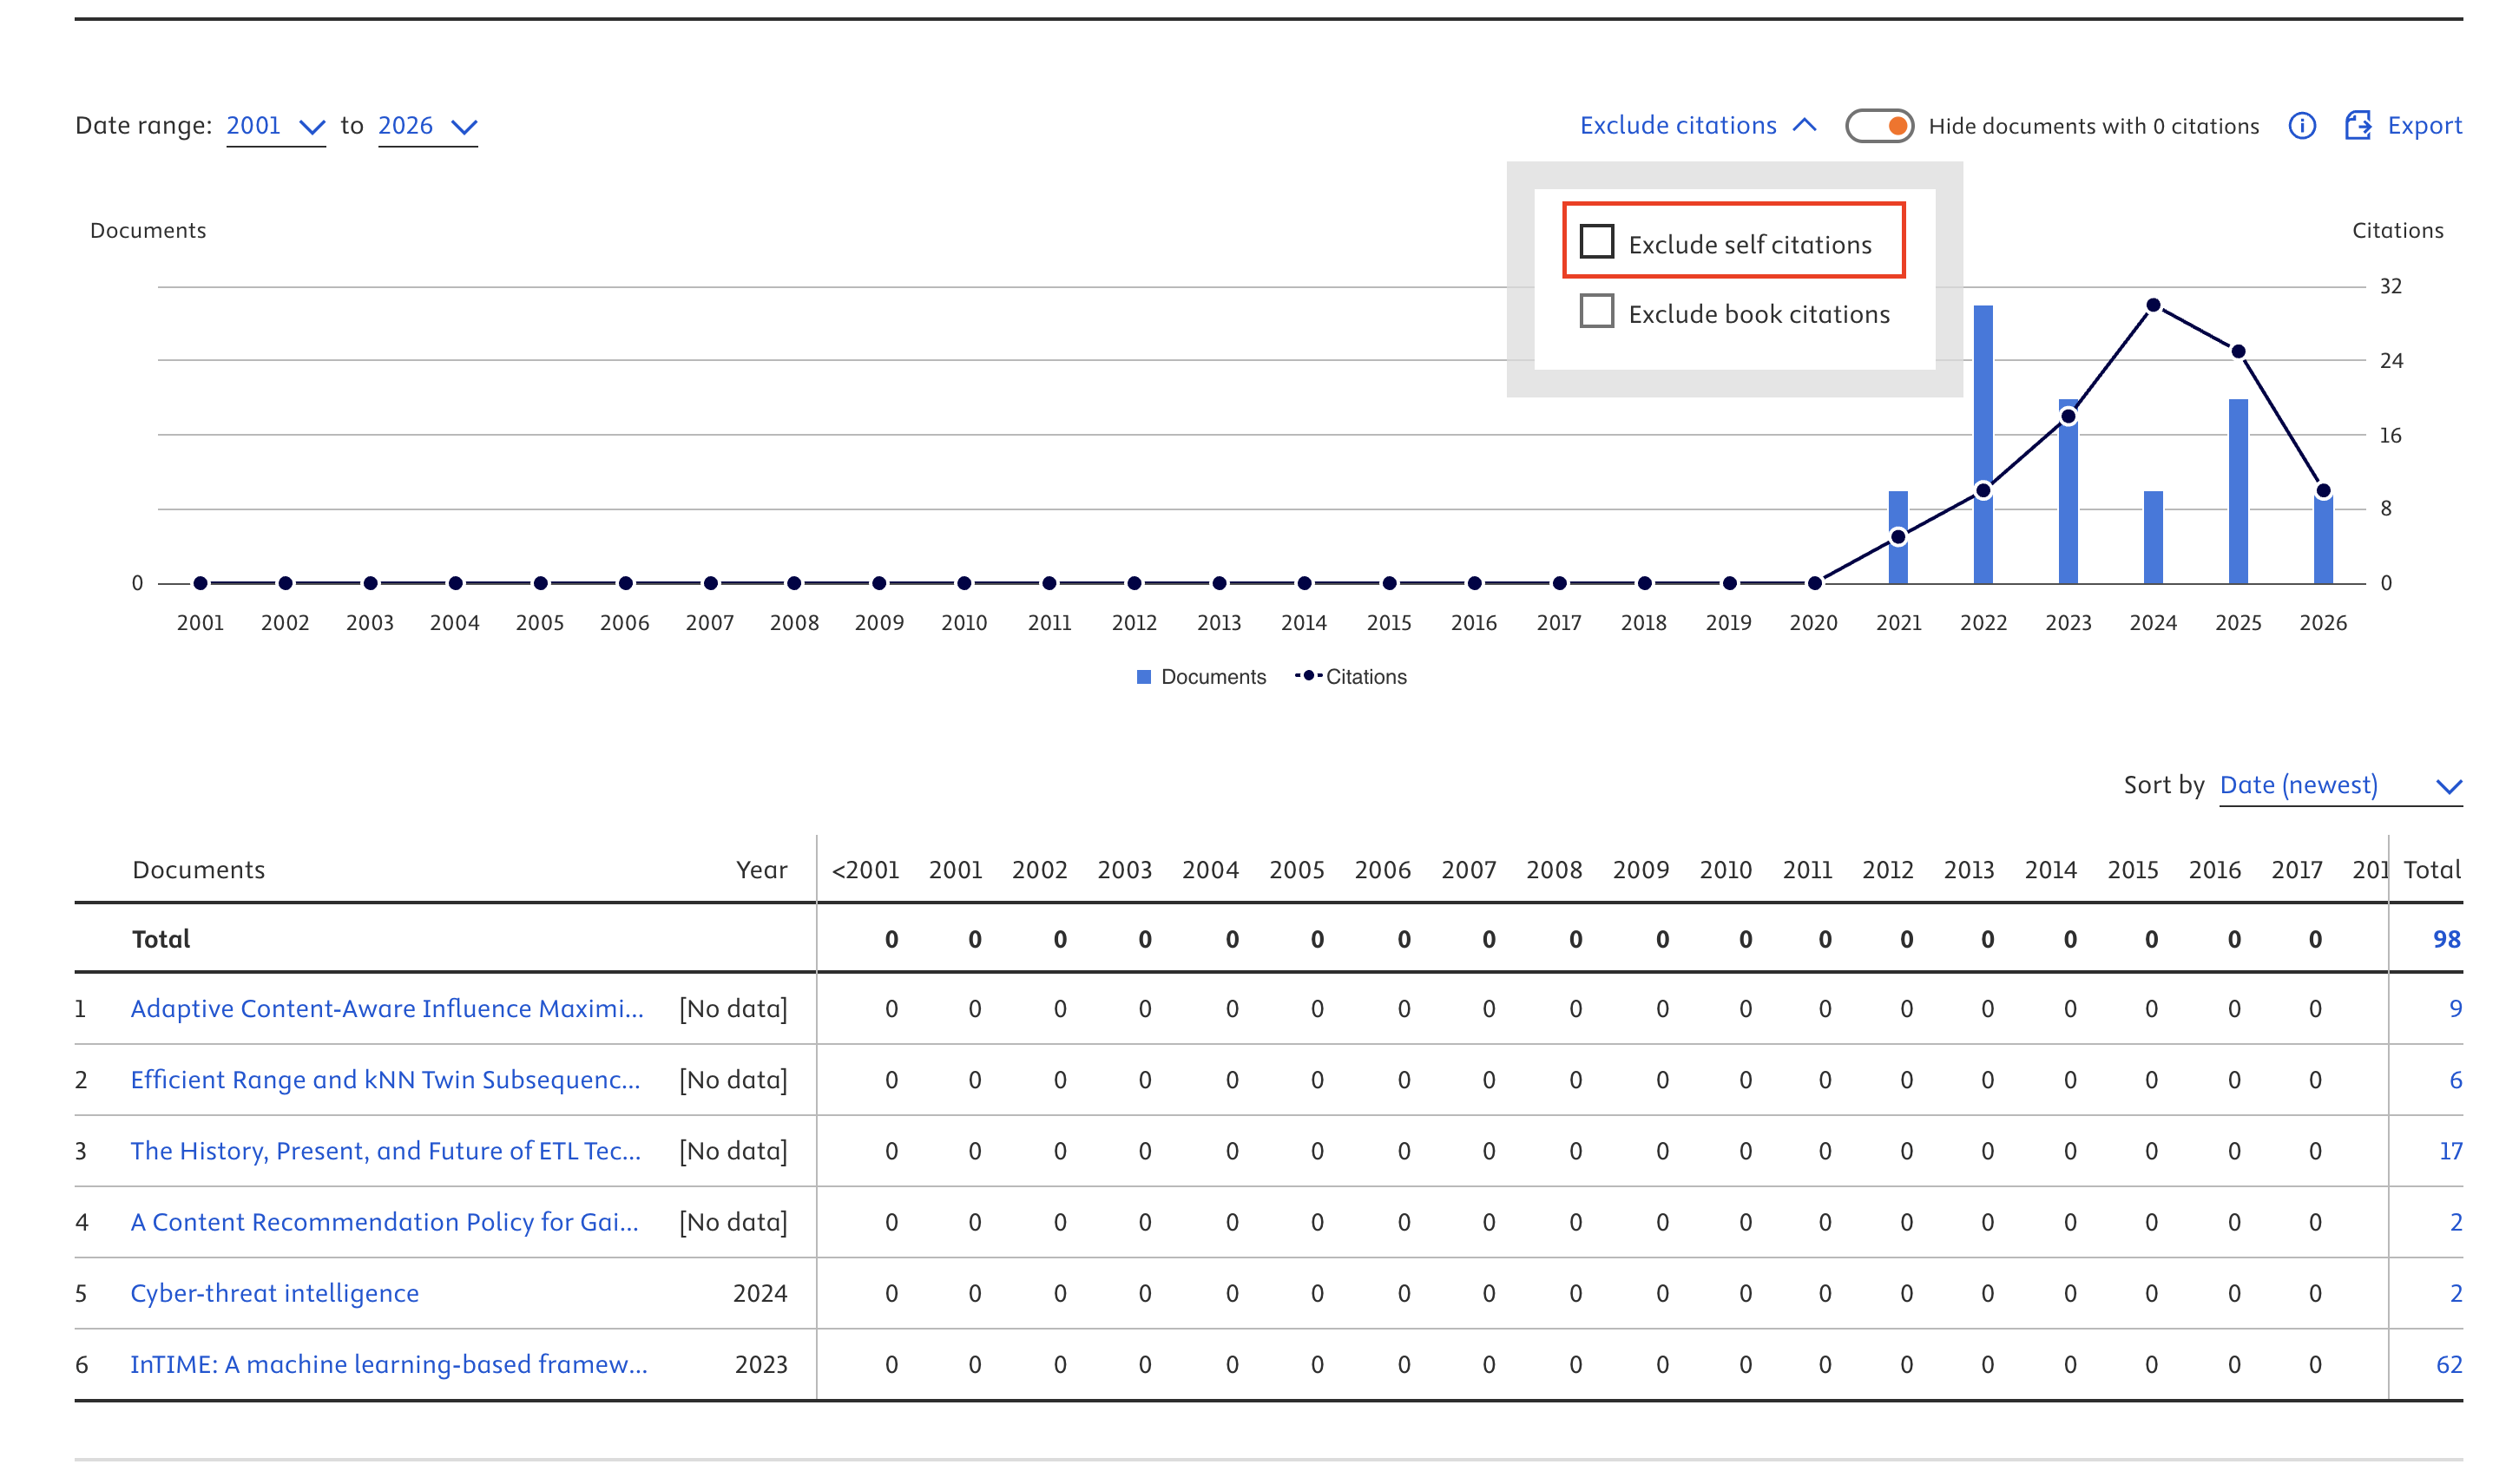
\includegraphics[scale=.3]{include/fig-scopus-2}
    \caption{Scopus interface allows to remove self-citations from the metrics}
    \label{fig:scopus-ui}
\end{figure}

\snote{You make too small paragraphs. An empty line in \LaTeX separates paragraphs. Typically, I use a single line for a paragraphs (despite the fact that intelij complains. You do not have to do like me. Yet a paragraph should have many sentences of a coherent content. You typically break the coherent content into many paragraphs. I corrected some, still keep this in mind.}
\enote{I find dense paragraphs harder to read. But I obviously can adapt and will do as you suggest.}

% !TEX encoding = UTF-8 Unicode
% !TEX root = ../Saunkin.tex


\chapter{Methodology} \label{c2:methodology}

The previous chapter presented an overview of existing systems and approaches to citation analysis.
These approaches rely on structured representations of publications and their relationships, typically in the form of citation networks.
This chapter introduces a data model representing publications and authors, and then proposes a methodology for distinguishing between self-citations and external citations.


\section{Data model} \label{sec:data-model}

The goal of the model proposed in this section is to define the minimum structure required for identifying and classifying citations.
Figure~\ref{fig:er-model} presents the data model used in this work; its entities and relationships are described below. 

\begin{figure}[tb]
    \centering
    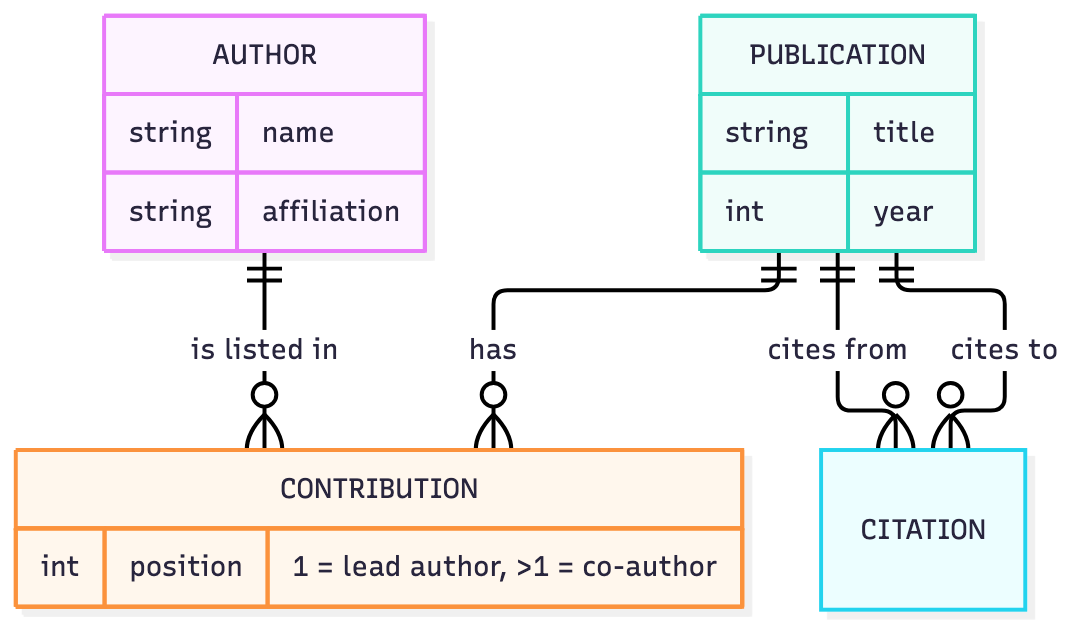
\includegraphics[scale=.2]{include/fig-data-model-er-diagram}
    \caption{Conceptual ER model for citation analysis}
    \label{fig:er-model}
\end{figure}

We identify two entities in the data of this system:

\begin{description}

    \item [Author] represents a researcher associated with one or more scientific publications.
    Each author is identified by the name listed in the publication.

    \item[Publication] represents a published scientific work.
    Each publication is described by a set of properties, forming a natural key: title, year of publication, and list of authors.

\end{description}

Two relationships are identified between the entities:

\begin{description}

    \item[Contribution] relationship connects authors and publications.
    A publication has one or more authors, and an author may write one or more publications (many-to-many).

    \item[Citation] represents a reference from one publication to another.
    A publication may cite and be cited by multiple other publications (many-to-many).

\end{description}

In addition to the contribution relationship, the author list (as it appears in the publication) is also retained as a property of the publication.
This reflects the way publications are usually identified, where author names form part of the citation string.
While the \emph{contribution} provides the structural relationship between authors and publications, the \emph{authors} attribute is used for identification.


\section{Classification of citations} \label{sec:citation-classification}

Based on the data model defined in the previous section, each citation can be classified by the relationship between the authors of the citing and cited publications.
The classification depends on whether the two publications share any authors.

A citation is classified as a \emph{self-citation} if at least one author appears in both the citing and the cited publication.
This definition is widely adopted in related studies, where self-citations are identified based on author overlap between publications~\cite{Glnzel2003BIBLIOMETRICSAA, Fowler2007}.
If the citing and cited publications do not share any authors, the citation is classified as an \emph{external citation}.

In addition to the basic distinction, self-citations can be further refined, to distinguish between citations made directly by the same author and those less strict, that arise naturally through citation of co-authored publications.
A citation is classified as a \emph{direct self-citation} of the author under analysis, if the author appears in both the citing and the cited publication.
A citation is classified as a \emph{co-author self-citation}, if the two publications share at least one author, but the author under analysis does not appear in the citing publication.

\section{Aggregation and processing pipeline} \label{sec:aggregation-pipeline}

The classification of citations is used to analyze citation behavior at the level of an individual author.

For a given author \(a\), the goal is to evaluate the citations received by the publications authored by \(a\), and to distinguish between different types of citations.

The process consists of the following steps:

\begin{itemize}
    \item All publications authored by \(a\) are identified.
    \item For each publication \(P_i\), all incoming citations are collected.
    \item These citations are classified according to the definitions provided in Section~\ref{sec:citation-classification}.
\end{itemize}

Following this process, the following counts can be evaluated for the author \(a\):

\begin{itemize}
    \item Total number of citations received by all publications authored by \(a\)
    \item Number of self-citations
    \item Breakdown into direct and co-author self-citations
    \item Number of external citations
\end{itemize}

Optionally, numbers produced by this pipeline can be evaluated against known metrics (e.g. Fi-score).

\section{Assumptions and limitations} \label{sec:assumption-and-limitations}

The methodology presented in this chapter assumes the availability of structured data describing publications, authors, and citation relationships.
In practice, the acquisition and quality of such data introduce several constraints.

\begin{itemize}
    \item Access to citation data is provided through external systems, typically imposing rate limits, which restricts the volume of data that can be retrieved within a time frame.
    \item Different sources provide inconsistent coverage of publications and metadata, which affects the quality of the citation graph.
    \item Identification of authors across publications is not uniquely standardized.
    Difference in naming and identifiers leads to ambiguity when determining whether publications refer to the same author.
\end{itemize}

These factors do not affect the formal definitions introduced in this chapter, but they influence the practical application of the methodology and are considered in the implementation described in the following chapter.

% !TEX encoding = UTF-8 Unicode
% !TEX root = ../Saunkin.tex

\chapter{Implementation and evaluation} \label{c4:implementation-evaluation}

This chapter discusses the implementation details and evaluates the results of the system, built following the methodology described in Chapter~\ref{c2:methodology}.
Section~\ref{sec:implementation} describes the architectural decisions, external connections, storage and caching mechanisms, overviews the processing flow, user interface, and other software development concerns.
Section~\ref{sec:evaluation} validates the outputs of the system, provides a few case studies, and compares data returned by each source.

\section{Implementation} \label{sec:implementation}

The system implements the citation analysis described in Chapter~\ref{c2:methodology}.
It takes an author name as input and returns citation counts, broken down into direct, co-author or external citations.
This section describes the component structure, data handling and processing steps to produce the results.

\subsection{System overview} \label{sec:system-overview}

There are two major use cases that the system attempts to satisfy.

\begin{description}
    \item[Author identification.] Select the unique author, whose citations user wants to examine.

    The initial search returns profiles matching the name provided.
    As the results can contain multiple entries matching the name, each item includes affiliations where available from the data source, or the user can request a list of publications, to help identify a particular author.

    The profiles are grouped by provider, as each source does not guarantee to use identifiers compatible with other sources.
    Matching a profile from one source to a profile from another would require a new algorithm to match identities, which is out of scope for this work.

    \item[Citation classification.] Having selected an author, collect all publications and incoming citations, classify them into the groups, to produce the aggregate counts.
    The backend compares author lists of each citing paper to classify citations according to the algorithm from Chapter~\ref{c2:methodology}.
    The results returned to the frontend contain counts and raw data.
\end{description}


\begin{figure}[tb]
    \centering
    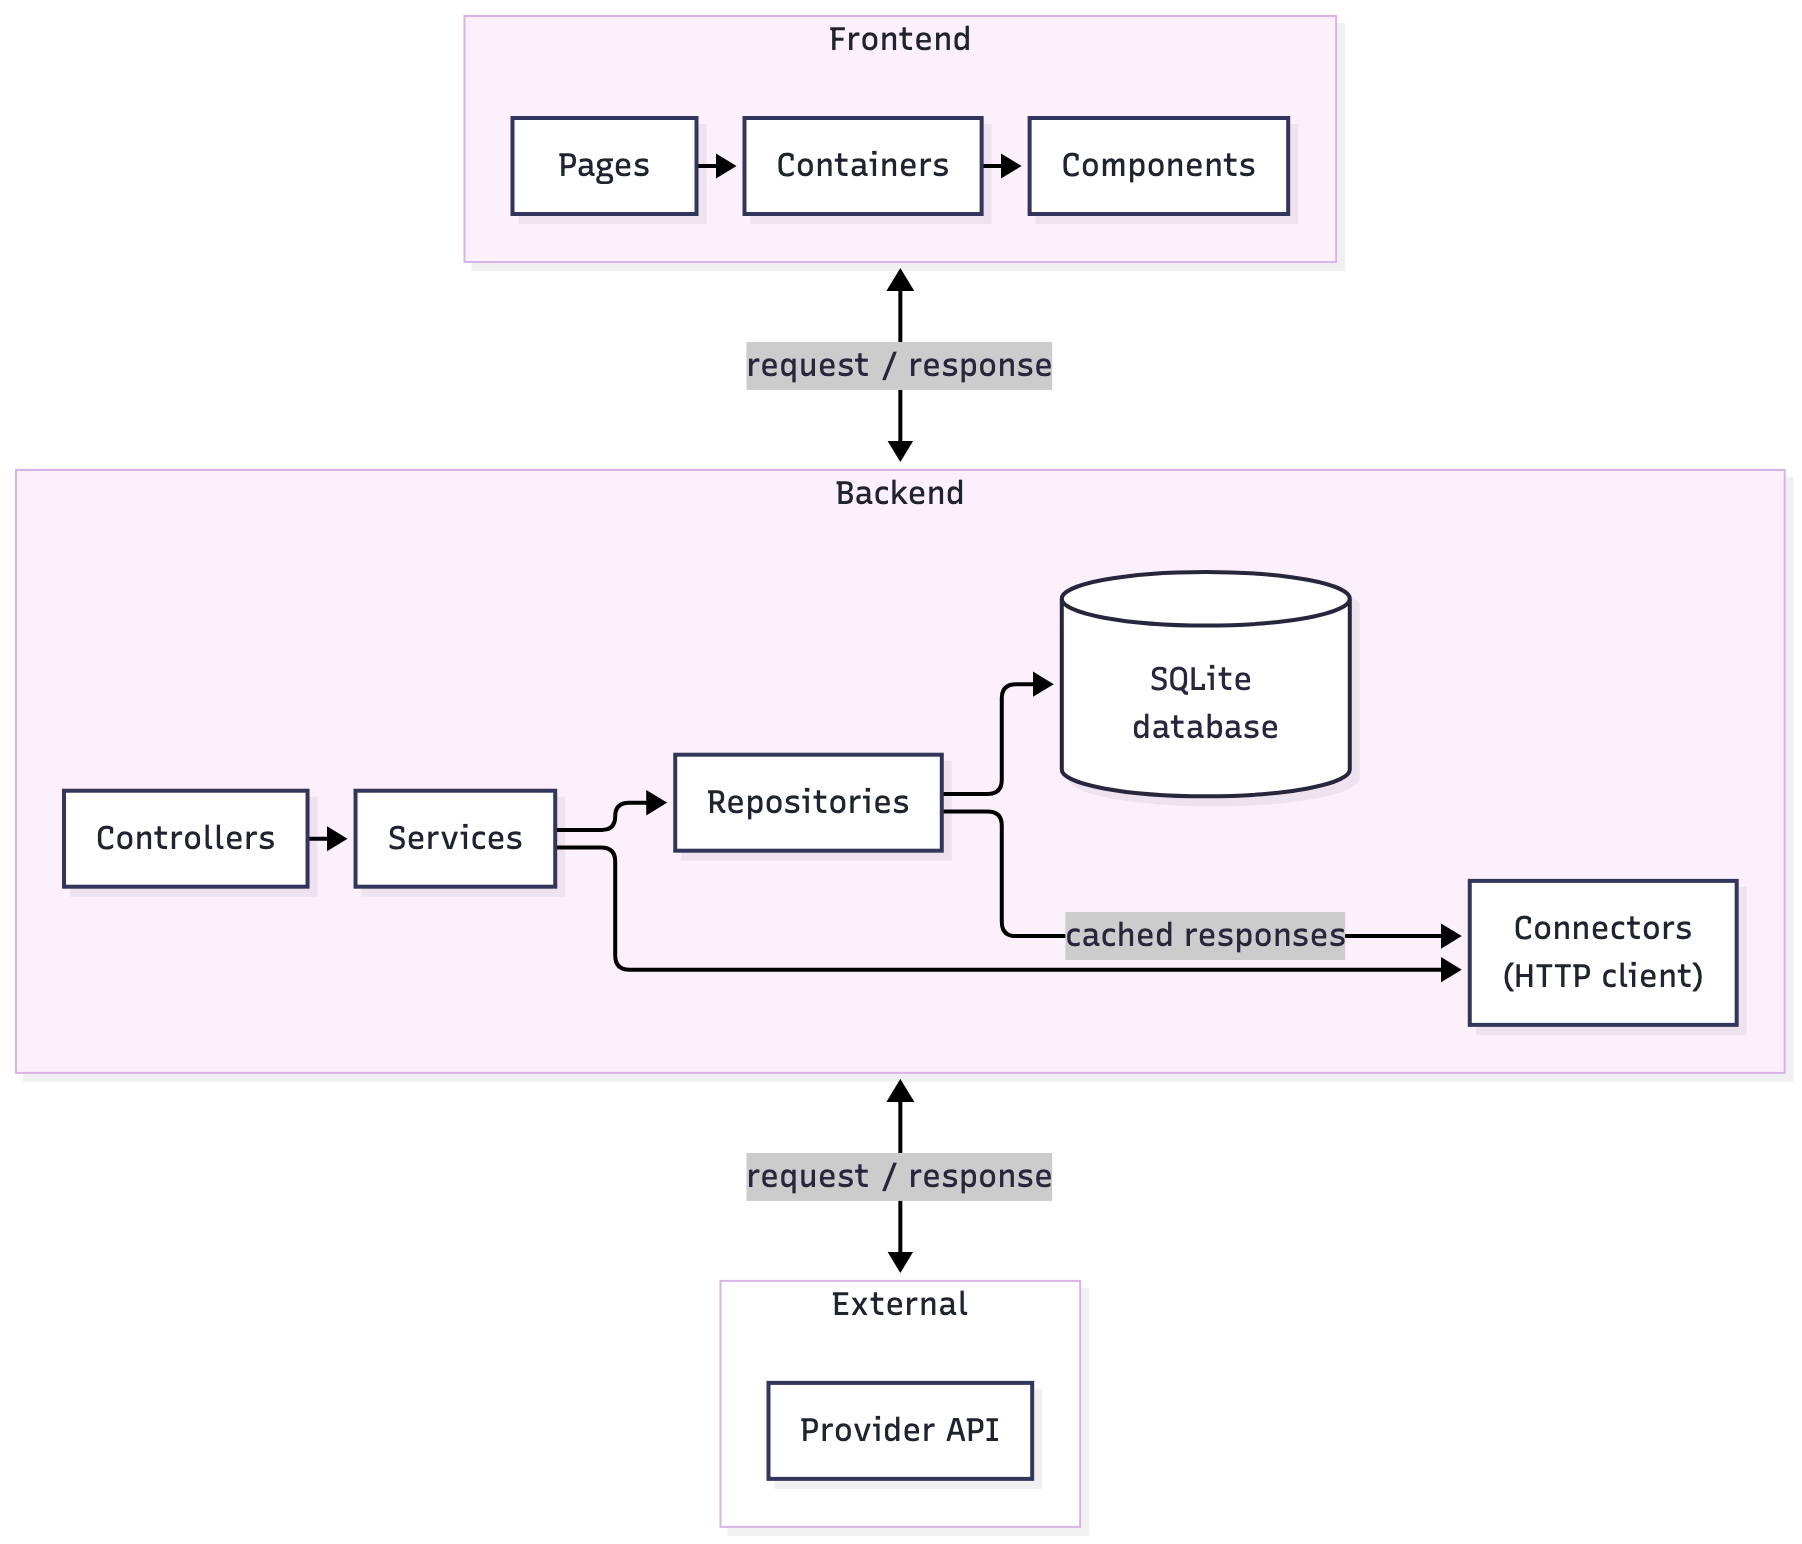
\includegraphics[scale=.2]{include/fig-arch-mvc-diagram}

    \caption{MVC architecture overview}
    \label{fig:mvc-pattern}
\end{figure}

The system design follows the Model-View-Controller (MVC) architectural pattern.
Figure~\ref{fig:mvc-pattern} outlines the architectural structure.


The user interface (UI) consists of a web page (frontend). 
It connects to the backend service, which encapsulates the business logic, and exposes the functionality via an Application Programming Interface (API).

Both system modules (frontend and backend) are written in \textsf{JavaScript}: the frontend is built with \textsf{React}, the backend targets \textsf{Node.js}.
The frontend does not implement any meaningful reusable business logic, instead it forwards the requests to the backend and displays the results.
The backend communicates with the external data sources to gather information, and performs citation analysis.

\subsubsection{Backend} \label{sec:backend-layers}

\snote{The backend consists of services, ... described as follows.}

\snote{See also what I have edited.}

\paragraph{Services} is the only component containing the business logic to coordinate the collection and analysis of data.

Services are classes corresponding to entity domains, exposing methods that provide the functionality expected of each entity.
They never see the request or the response objects.
Instead, they receive transformed and sanitized arguments, and return data structures corresponding to their own internal model.
This separation keeps the business logic independent of the transport protocol: the same service can be invoked by a controller, injected into another service, or unit tested.
There is one service for each subject:
\begin{enumerate}
\item
\textsf{AuthorService} for author profiles, 
\item
\textsf{PublicationService} for papers and citations, 
\item
\textsf{ClassificationService} for the classification algorithm, 
\item
\textsf{CitationGraphService} for operations on the citation graph as a whole, 
\item
\textsf{JobService} for the background jobs, and 
\item
\textsf{MetricsService} for the count aggregation.
\end{enumerate}

Dependencies are injected into each service to provide the underlying functionality needed to produce the results.
For instance, the \textsf{MetricsService} orchestrates the flow to produce the citation collection described in Section~\ref{sec:processing-pipeline}: it requests the papers of the selected author by calling the \textsf{AuthorService}, the citations of each paper through the \textsf{PublicationService}, and the classification of each citation through the \textsf{ClassificationService}, to finally hand the assembled graph to the \textsf{CitationGraphService} to be stored.

\paragraph{Connectors} handle the fetching and processing of data from external sources.

Connectors are also classes, one per provider, implementing the communication with external data sources; no other component is allowed to contact a provider directly, instead all requests for external data go through the connectors.
Every connector implements the same interface (\textsf{ProviderConnector}) with the operations described in Section~\ref{sec:providers}, so the rest of the system treats all sources in the same manner.

A connector transforms the responses into the internal model, that is used by the rest of the system.
All provider specifics are isolated inside the respective connector: the endpoint structure, the request and response models, pagination, authentication etc.
For instance, the \textsf{OpenAlex} connector paginates with 200 records per page, and the \textsf{Google Scholar} connector is limited to 20 records per page; both return the same data structure, regardless of how they gather the results.

\paragraph{Controllers} receive user requests and pass them to services.

Controllers are classes with one method for each API endpoint that the backend exposes.
They contain minimal business logic, limited to the endpoint structure, as a function of the interface that the service provides.
Their responsibility is to validate the incoming parameters, transform the requests into the internal model, call the respective service, transform the service result into a response.
For instance, a search request without a query parameter is rejected with a status code \textsf{400}, not having reached a service.
Controllers are separated by the use cases.
There is \textsf{SearchController} for the author search, \textsf{AuthorController} for the author details, papers and stored metrics, \textsf{JobController} for submitting jobs and polling their status, and \textsf{StatusController} for the provider quotas and system resources.

\paragraph{Repositories} read from and write to the database tables.

Repositories, too, are classes with methods, implementing the functionality that depends on connection to the database; no other component is allowed to make database queries directly, instead all requests for data go through the methods exposed by the repositories.
There is one repository for each table: \textsf{publications}, \textsf{authors}, \textsf{contributions}, \textsf{citations}, \textsf{cache} and \textsf{jobs}.

Repositories implement only the SQL operations that the application needs, not every possible operation on every table.
They expose arbitrary methods, for instance to save items or to find records by different criteria.

Instead of writing the queries directly in SQL and sending them through the database driver, the repositories use an object-relational mapping (ORM) library (\textsf{Drizzle}\footnote{\url{https://orm.drizzle.team}}).
The schema of tables and columns is declared in code, as described in Section~\ref{sec:storage-caching}, and the queries are expressed as code as well, to allow this layer of the system to be statically analyzed and unit tested, just like the rest of the project.

As the repositories are isolated per entity, only the relevant repositories are injected into the respective services.
For instance, the citation graph service (\textsf{CitationGraphService}) needs to read and update the tables \textsf{publications}, \textsf{authors}, \textsf{contributions} and \textsf{citations} to save a collected graph and load it back, so the four respective repositories (\textsf{PublicationRepository}, \textsf{AuthorRepository}, \textsf{ContributionRepository}, \textsf{CitationRepository}) must be provided in the constructor.

\subsubsection{Frontend} \label{sec:frontend-layers}

The frontend serves as a presentation layer and interface controller, and follows a data flow similar to the backend.
The building blocks of the UI are \emph{components}, \emph{containers}, and \emph{pages}.

\begin{figure}[tb]
    \centering
    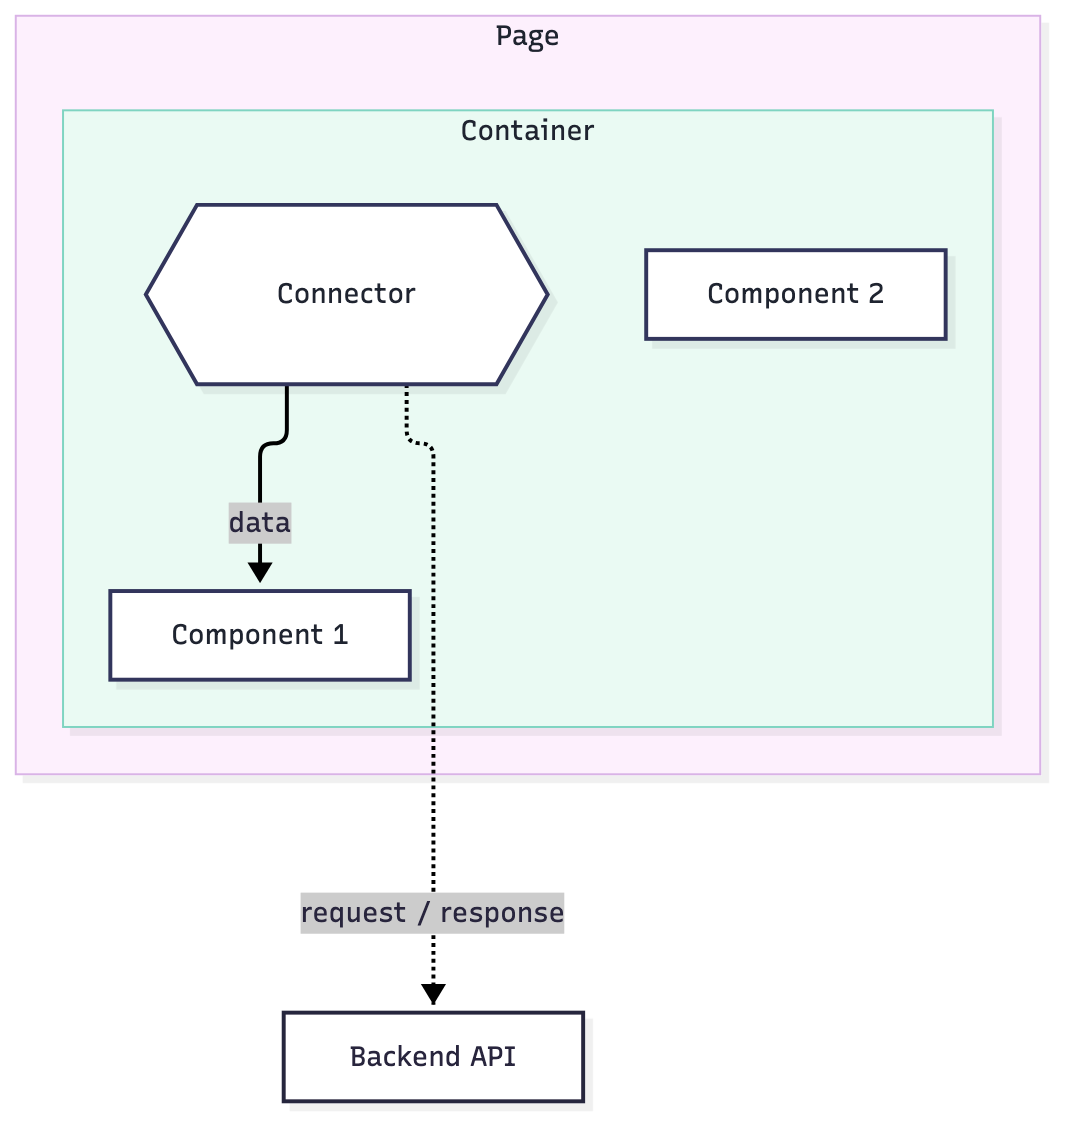
\includegraphics[scale=.2]{include/fig-frontend-component-diagram}

\snote{This might be a nice scale. Still there is unnecessary space between the shapes. Mermaid is not very configurable}

    \caption{Frontend building blocks: pages, containers and components}
    \label{fig:frontend-components}
\end{figure}

Figure~\ref{fig:frontend-components} shows how the frontend is composed and how it connects to the backend. \snote{This is right. Still, you need to discuss the figure.} \enote{done}

\emph{Components} are the reusable atomic widgets that define how a piece of data should look and behave.
They are not responsible for retrieving the data, only for rendering and styling it.
For example, a loading indicator or an error message are components, and can be used on different occasions by different containers.

\emph{Containers} are meaningful groups of related components.
They manage and request data, implement all the presentation logic around orchestration of the components.
They are responsible for calling the API, showing the loading or error state, as well as wiring together the components and supplying the data to them.

\emph{Pages} are the largest units of the frontend, each page usually corresponds to a unique path of the address in the browser.
The application currently consists of two pages: author search (\texttt{/authors}) and author details (\texttt{/author/:provider/:authorId}).
Each page is built with one or more containers.

The backend performs the retrieval as an asynchronous background job, to provide progress while collecting data, which can potentially take time, especially for authors with many publications and sources with low throughput.
The frontend polls and displays the progress of these jobs in the UI.

The following sections describe the provider choices, data model and processing steps in more detail.

%\enote{done (mermaid is my tool)} \snote{Fine, but also put the sources in the repo. } \enote{done (previously they were all in the system-design.md, extracted also into docs/fiagrams; build by `make diagrams`)}

\subsection{Providers and limitations} \label{sec:providers}

Citation sources were analyzed in Section~\ref{sec:data-sources} by the supported data properties and the provided access methods (see also Figure~\ref{fig:providers-overview}). Among these, three data providers were supported in our system implementation: \textsf{OpenAlex}\footnote{\url{https://openalex.org}}, \textsf{Semantic Scholar}\footnote{\url{https://www.semanticscholar.org}}, \textsf{Google Scholar}\footnote{\url{https://scholar.google.com}} (via \textsf{SerpApi}\footnote{\url{https://serpapi.com}}).

\textsf{OpenAlex} and \textsf{Semantic Scholar} are the most naturally fitting open sources.
Their responses to requests for citations also include author lists, needed by the classification algorithm.
\textsf{Google Scholar}, as the one with the widest coverage, was also considered, despite all the limitations around using it.
The remaining sources were not considered:

\begin{description}
    \item \textsf{CrossRef}\footnote{\url{https://www.crossref.org}} does not list the citing papers.
    \item \textsf{OpenCitations}\footnote{\url{https://opencitations.net}} does not support search by author name (only by identifier).
    \item \textsf{DBLP}\footnote{\url{https://dblp.org}} is limited to computer science and does not provide citations.
    \item \textsf{Scopus}\footnote{\url{https://www.scopus.com}} requires a paid institutional subscription.
\end{description}


%Figure~\ref{fig:providers-overview} shows the provider connectors.

\begin{figure}[tb]
    \centering
    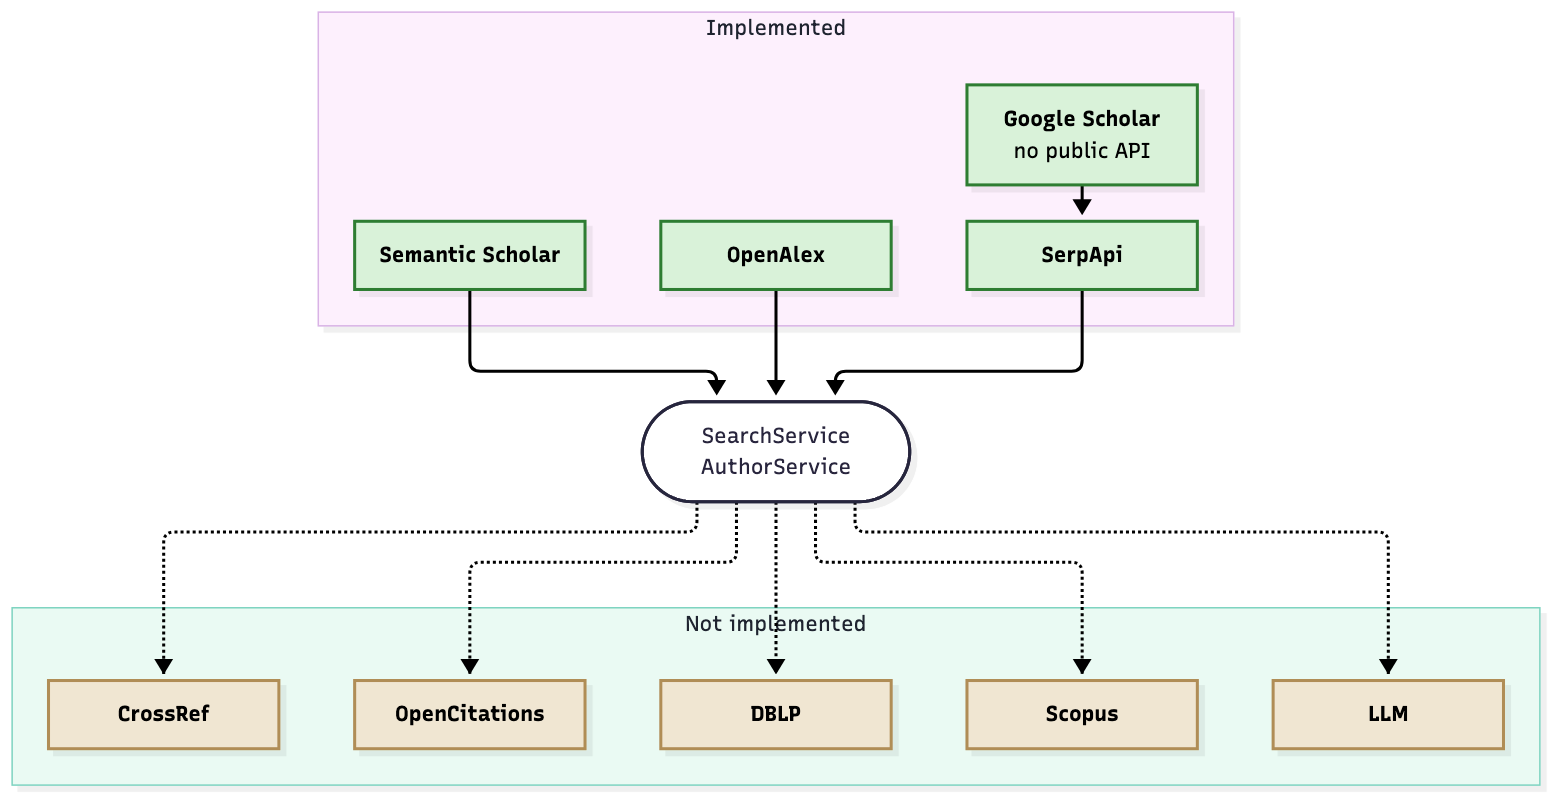
\includegraphics[scale=.2]{include/fig-providers-diagram}
    \caption{Providers and their respective connectors}
    \label{fig:providers-overview}
\end{figure}

In the backend, each data source is reached through its own \emph{connector}, to isolate the differences in access and the structure of data it returns.
Every connector implements the interface \textsf{ProviderConnector}, defining the operations:

\begin{description}
    \item \textsf{searchAuthors} to find an author,
    \item \textsf{getAuthorPublications} to list author papers,
    \item \textsf{getCitations} to list paper citations.
\end{description}

The remaining system builds on top of these operations, treating all sources in the same manner.
As the connectors are interchangeable, a source may be added or replaced without changing the remaining processing pipeline.
At the same time forensic bug investigation for each source remains within its own connector, making it easy to locate problems and test behavior.

Each provider imposes a concurrent request throttling.
The implementation uses asynchronous queues to stay within the rate limits.

None of the sources considered for this project shares author identifiers fully compatible with another.
The profiles are kept separate and shown side by side, as described in Section~\ref{sec:system-overview}.

The largest source (\textsf{Google Scholar}), even when accessed via a paid proxy (\textsf{SerpApi}), is the most restrictive in practice.
Collecting the citations of an author with $n$ publications requires at least $n$ requests, growing the cost proportionally to the volume of data retrieved.
The free sources (i.e., \textsf{OpenAlex} and \textsf{Semantic Scholar}) are used by default in the system.

\subsection{Data} \label{sec:data}

The conceptual model described in Section~\ref{sec:data-model} translates to four domain-specific tables: \textsf{authors}, \textsf{publications}, \textsf{contributions}, and \textsf{citations}.
There is also a table to save the asynchronous jobs state (\textsf{jobs}), and a table for cached responses (\textsf{cache}), described in Section~\ref{sec:storage-caching}. \snote{You might need to present them in a figure. The ER maybe?} \enote{done}
Figure~\ref{fig:database-er} shows the database tables and the relationships between them.

\begin{figure}[tb]
    \centering
    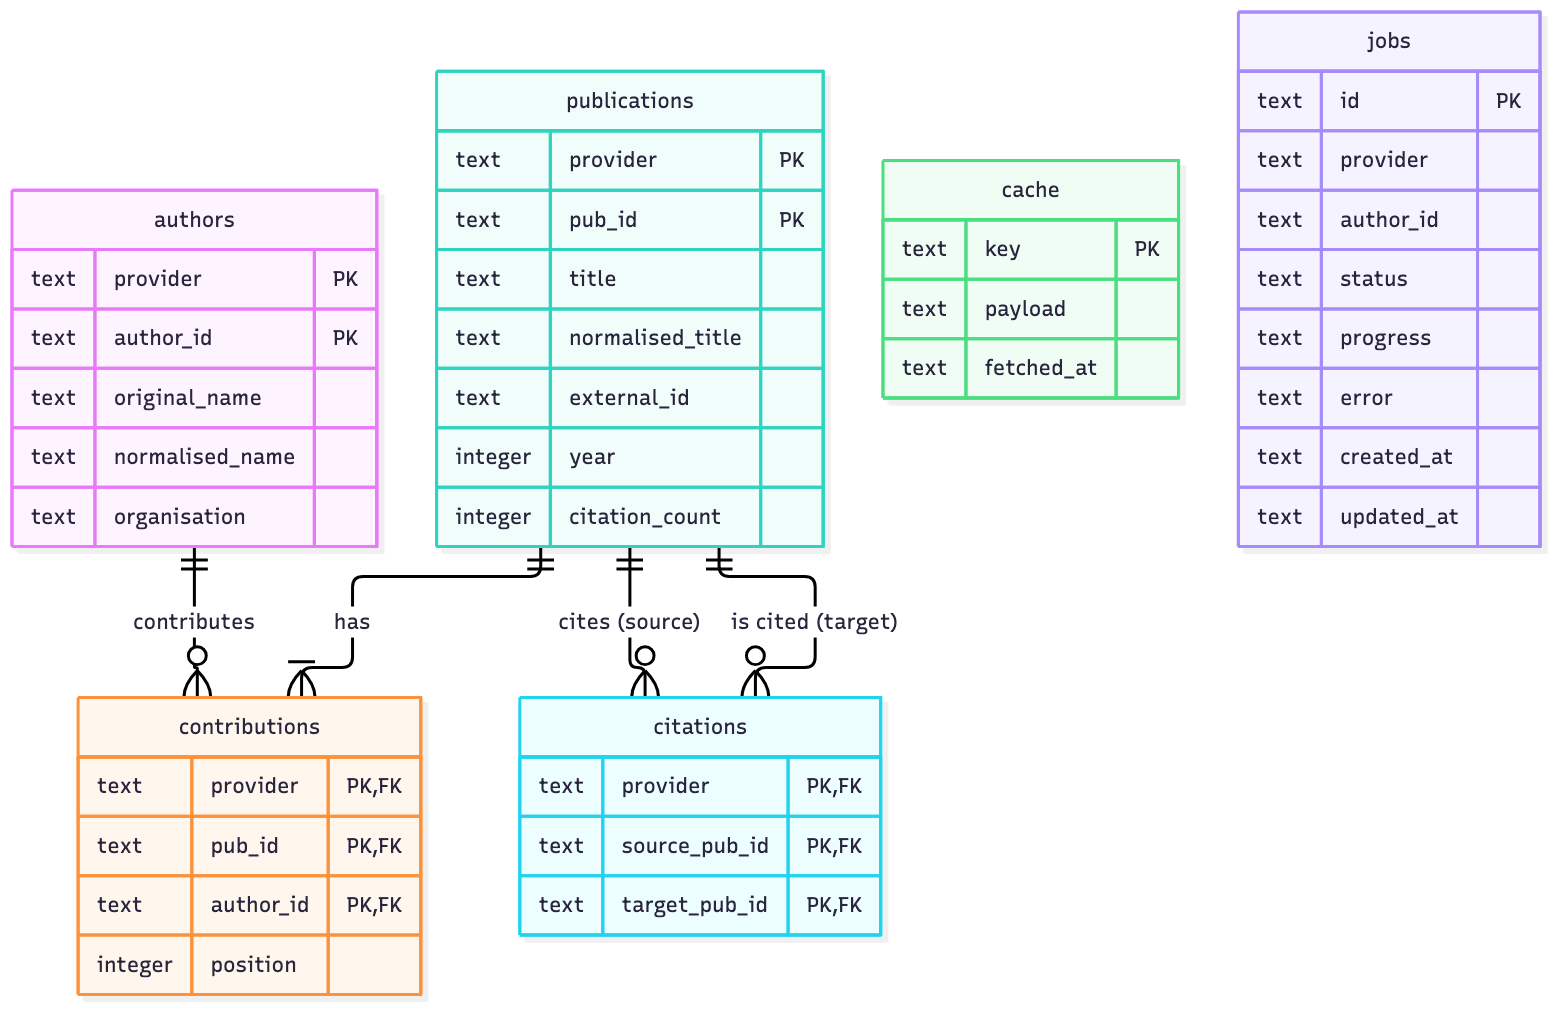
\includegraphics[scale=.2]{include/fig-database-er-diagram}
    \caption{Database tables}
    \label{fig:database-er}
\end{figure}

In the conceptual model, a publication is identified by its title, year and authors, and an author by name.
The implementation uses the identifiers assigned by each provider: \textsf{pubId} and \textsf{authorId}.
Names and titles can be ambiguous, and spelling differences do not necessarily mean that two records refer to different entities.
All primary keys are composite and include the provider identifier.
This is necessary to keep the data separate by provider.

A \textsf{publication} record contains the title, year, citation count reported by the provider, and an external identifier, for instance a DOI, if available.
An \textsf{author} record consists of the name and the affiliation, if available.
A \textsf{contribution} record connects an \textsf{author} to a \textsf{publication}; it includes the position of each one of the list of paper authors.
A \textsf{citation} record connects the \textsf{citing publication} (source) to the \textsf{cited publication} (target).

Normalized author names and paper titles are stored in the respective entity tables, alongside the original names and titles.
The normalization consists of simple string manipulations, such as conversion to lower case, removal of diacritics, and replacement of repeated whitespace.
For example, ``Skiadópoulos'' and ``skiadopoulos'' produce the same normalized value.

\textsf{OpenAlex} and \textsf{Semantic Scholar} typically return authors and publications with their own internal identifiers.
Their connectors filter the list of contributions to remove ones without an author identifier.
The \textsf{Semantic Scholar} connector also discards citing papers without a paper identifier.

\textsf{Google Scholar} does not guarantee to return identifiers for the authors of citing papers, often it returns names as strings, which are inherently unreliable for uniquely identifying anything.
When an identifier is missing, the respective connector uses the normalized name, but this remains a known issue, leading to self-citations being potentially under-represented in the \textsf{Google Scholar} results.

\subsection{Storage and caching} \label{sec:storage-caching}

\textsf{SQLite} was used in the system for the simplicity of its setup.
It does not require a separate server, instead it runs within the backend process and stores the database in a single file.
Schema changes \snote{I am not sure what you mean. It seems nice and important. Give it more space} \enote{done} also live in the codebase: they are defined as migrations and applied at runtime, every time the database is opened by the backend process.

The schema is only defined in code, in a single file describing every table.
When the schema changes, the ORM compares it with the previous version and generates code representing the migration.
A migration is a file with SQL statements needed to change the current database schema to the new schema.
Migrations are kept in the codebase and are checked into the version control system.
Every time the backend starts up and opens the database, it applies the migrations that have not been applied yet.
Using this approach, the database schema always starts from the initial empty state, it then grows, and eventually evolves into the final version of the schema needed by the application.
By keeping the database schema in the repository, the domain model changes can be associated with the current application model, to keep the models synchronized.

The system largely depends on externally sourced data, subject to the provider limitations and the latency of network access.
Publications, authors, contributions and citations are treated as immutable in nature.
These details, when retrieved and linked together, form a graph of nodes and relationships, coined as \textsf{citation graph}. \snote{Describe it, which are the nodes, which are the edges, which are the semantics. } \enote{done}

The citation graph is a two-dimensional representation of the conceptual domain model.
In this graph, \emph{publications} and \emph{authors} are the nodes of this graph, \emph{contributions} and \emph{citations} are the two types of directed edges.

The graph can be pivoted to center around any author, producing three levels of layering.

\begin{description}
    \item [Selected author] is connected to their own papers (as \emph{contributions}).
    \item [Citing papers] are connected to the selected author papers (as \emph{citations}).
    \item [Citation authors] are connected to each citing paper (as \emph{contributions}).
\end{description}

The citation graph is decomposed and stored as separate entities in the tables
\textsf{publications}, \textsf{authors}, \textsf{contributions} and \textsf{citations} (Figure~\ref{fig:database-er}), as described in Section~\ref{sec:data}.  \snote{Name the tables and give a pointer to the respective figure.} \enote{done}

The citation graph described in Section~\ref{sec:user-interface} represents the citations graph visually.

After collecting the data, the backend saves the publications, authors and their relationships, from which the graph can be reconstructed without network requests to external providers.
Classification labels depend on the choice of author (the same citation can be \textsf{direct} for one author and a \textsf{co-author self-citation} for another) and are calculated at runtime, when the graph is loaded. \snote{I am not sure that I get it. Why don't you give an example and a figure?} \enote{done}

Figure~\ref{fig:classification-example} shows the classification of the same citation for different authors, involved in either or both of the papers.

As an example, let us consider the publications discussed in Chapter~\ref{c1:intro}.
[KGMP2007]~\cite{Kalnis2007} by Kalnis, Ghinita, Mouratidis and Papadias cites [GPK2007]~\cite{Ghinita2007} by Ghinita, Kalnis and Skiadopoulos.
The citation classification changes depending on who is the author under analysis.
For \emph{Kalnis} or \emph{Ghinita}, as authors of both papers, the citation classification is \textsf{direct self-citation}.
If the selected author is \emph{Skiadopoulos}, who only appears on the cited publication, the classification cannot be \textsf{direct self-citation}.
As other authors of the cited paper also appear on the citing paper, the classification is then \textsf{co-author self-citation} for Skiadopoulos.

\begin{figure}[tb]
    \centering
    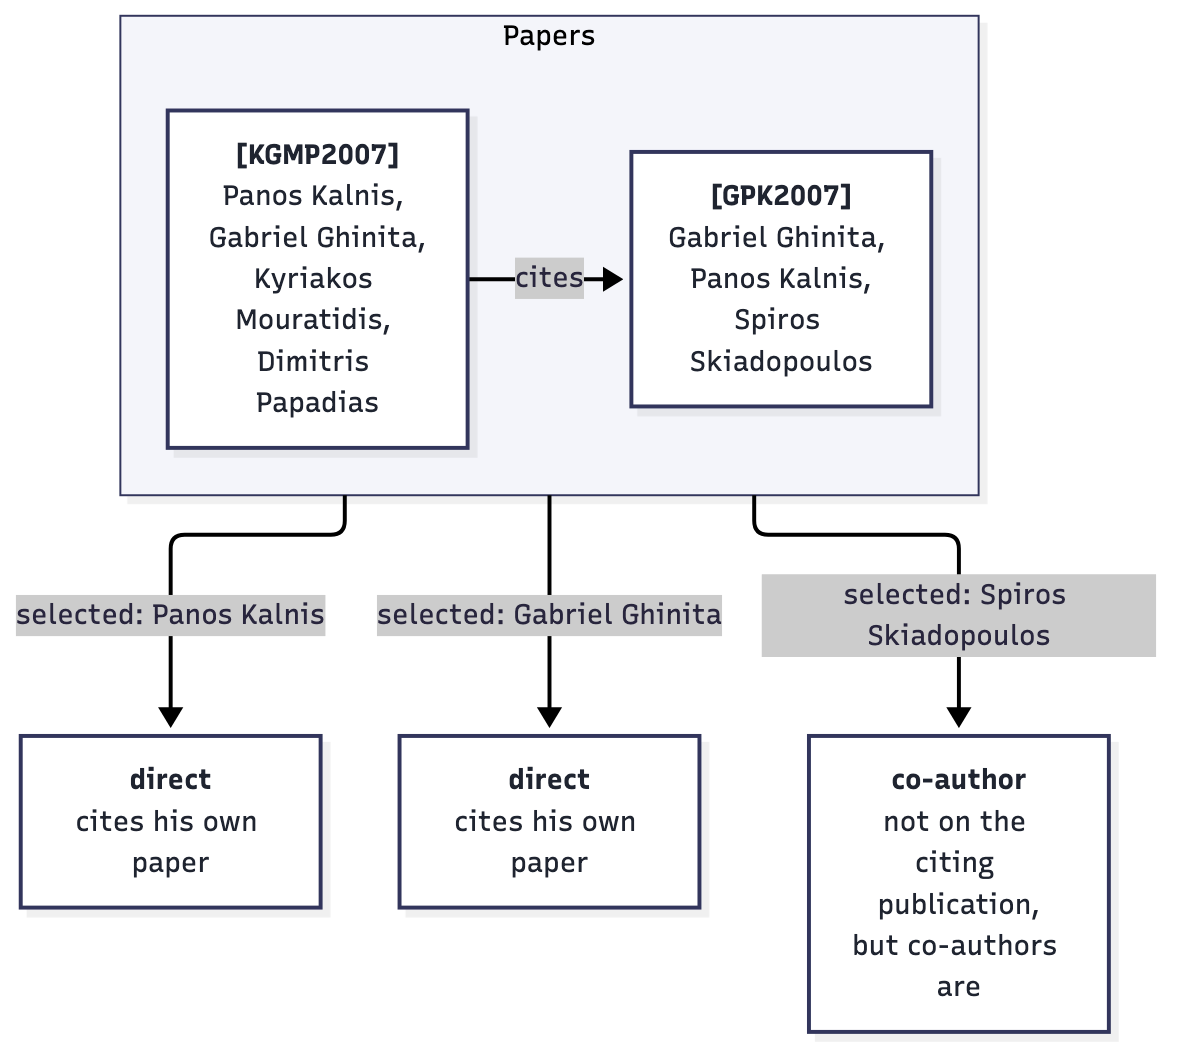
\includegraphics[scale=.2]{include/fig-classification-example-diagram}
    \caption{Classification of the same citation for each selected author}
    \label{fig:classification-example}
\end{figure}

Figure~\ref{fig:cache-flowchart-diagram} illustrates the data flow inside the cache mechanism. \snote{You start with this. Give the pointer to the Figure and then discuss the figure. Not vice-versa. }\enote{done}
All provider connectors use the same HTTP client implementation, with caching handled internally.
Before sending a request, the client looks for a stored response using the request URL as the key.
The cache key enforces the order of the query parameters alphabetically, to provide a stable key, regardless of the parameter order in the original request URL.
For instance, \texttt{https://example.com?p1=v1\&p2=v2} \snote{use verb, texttt or url do not use quotes.}\enote{done} and \texttt{https://example.com?p2=v2\&p1=v1} produce the same key.
Each cached record includes the date it was received, used to calculate whether the record satisfies the time-to-live timeframe.

\begin{figure}[tb]
    \centering
    \snote{see the comments for the figures above.} \enote{done}


    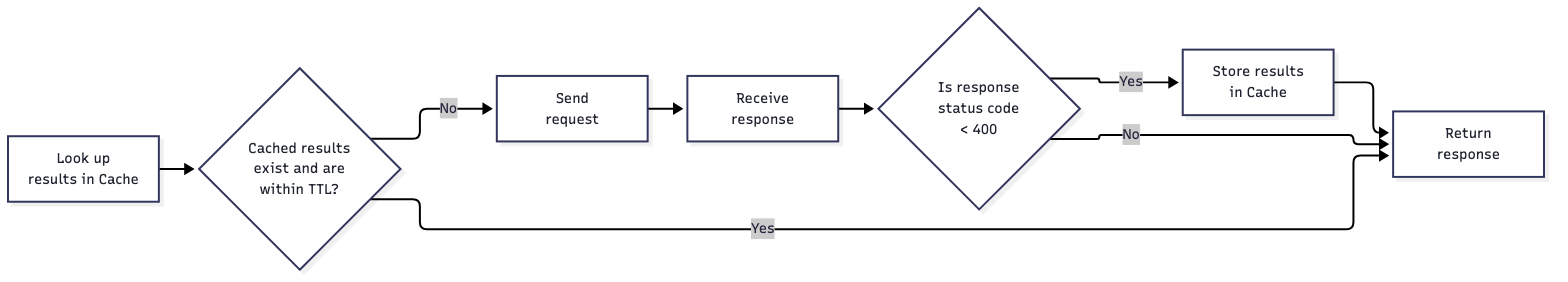
\includegraphics[scale=.3]{include/fig-cache-flowchart-diagram}
    \caption{Cache request data flow}  

    \label{fig:cache-flowchart-diagram}
\end{figure}

If the record is found, and it has not expired, the response contained within is returned; otherwise, the request is sent to the provider.
Successful responses are stored as text under the same key and with the current date.

Expired cache records are replaced when requested again, but there is no periodic deletion of old entries, and there is no limit on the cache size.
The database can grow forever, which is a limitation of a shared installation, that would need a retention policy and clean up procedures.

\subsection{Processing pipeline} \label{sec:processing-pipeline}

Once the user has selected the author, the UI automatically checks whether a citation graph for this author exists in the system for the currently selected provider, using the date of the last completed job for this author and provider, which the backend returns with the author details.
If the citation graph exists, it is returned as a raw dataset in JSON format, and that date is shown as the time of the last update.
The UI renders results, including an option to update the results, bypassing the previously stored graph and cache.
If the citation graph does not exist, or the user has requested to update the results, the backend receives a request to fetch the full graph.

Having received a request to fetch the full graph from a provider, the backend creates a new job (as an in-memory object) and stores it in the database.
The job is initially placed in the state \textsf{running}, which is the only non-final state.
The backend immediately responds with the job object, including the identifier.
With the identifier at hand, the client starts to poll the job status, until it reaches one of the final states: \textsf{done}, \textsf{error}, or \textsf{interrupted}.

Meanwhile, in the background, the backend orchestrates the flow to build the citation graph.
Figure~\ref{fig:classification-flowchart-diagram} illustrates the data flow of constructing the full graph from an author identifier.
The successful path is as follows:

\begin{itemize}
    \item The \textsf{Metrics service}, which orchestrates the flow, hands it over to the \textsf{Author service}
    \item The \textsf{Author service} requests the list of papers for the selected author identifier, and paginates to reach the end of the response list
    \item Having reached the end of the list, the \textsf{Author service} calls the \textsf{Publication service} to fetch the citations, for each of the gathered publications
    \item The \textsf{Publication service} requests the list of citations, and extracts the authors from each item of the list
    \begin{itemize}
        \item In practice, the requests for all publications are sent at once, and the provider request queue paces them to the number of requests per second that the provider allows
    \end{itemize}
    \item Having gathered details of each of the citing publications, the control returns to the \textsf{Metrics service} to aggregate final results
    \item The \textsf{Classification service} applies the classification algorithm to each of the citing publications against the currently selected author, and finally
    \item The \textsf{Metrics service} collates the results into a single nested structure, stores it in the database, and changes the job status to \textsf{done}
\end{itemize}

If the citations of a publication cannot be retrieved, for instance due to a network error, this publication is skipped, but the job still completes.
The result mentions how many publication responses were successful and how many failed.

Once the job has been updated with the final result, the next time the client requests the job, it will receive the result and will be able to fetch it and render in the UI.

\begin{figure}[tb]
    \centering
    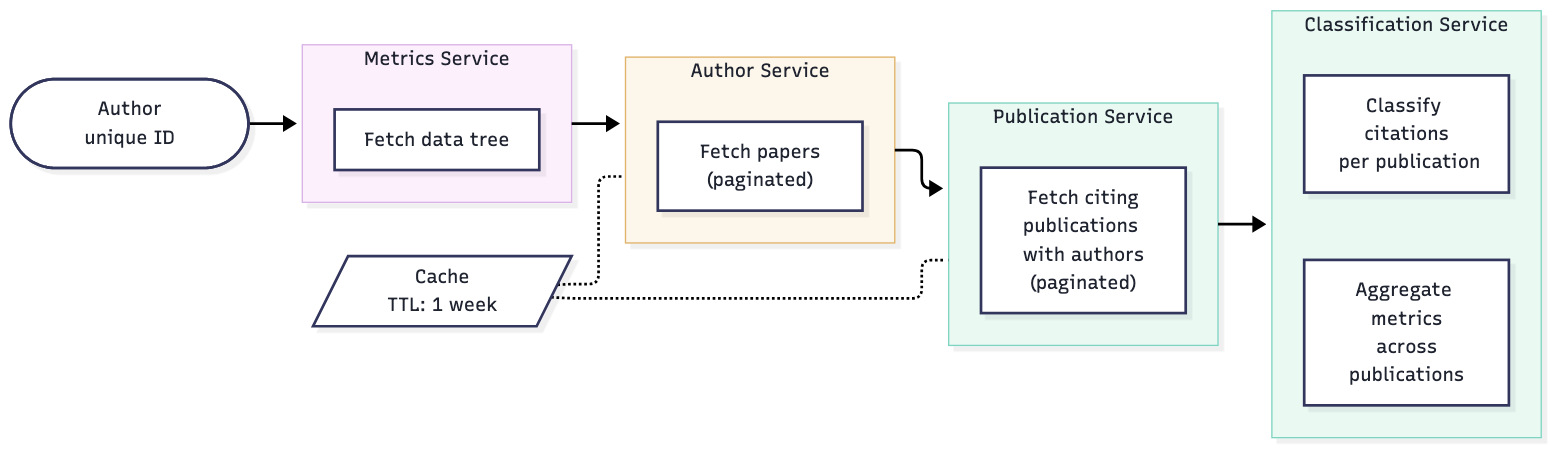
\includegraphics[scale=.3]{include/fig-classification-flowchart-diagram}
    \caption{Citation graph construction data flow}
    \label{fig:classification-flowchart-diagram}
\end{figure}

\subsection{User interface} \label{sec:user-interface}

The software application responsible for interaction with the user, user interface (UI), consists of a single-page web application.
User interface addresses the use cases described in Section~\ref{sec:system-overview}: finding an author, and getting citation metrics for a selected author.
The application consists of a few individual components described below: \textsf{Search form}, \textsf{Search results}, \textsf{Author details}, \textsf{Status}.

\subsubsection{Search form} \label{sec:ui-search-form}

Figure~\ref{fig:ui-search-form} shows the initially empty search page, where the user enters a name to start the flow of selecting an author.
Currently, there is no way to disable or enable some of the providers, this setting is controlled by the backend.

The page supports deep-linking to the search form with the name prefilled, when the URL specifies the parameter \emph{q=query}, for instance \texttt{http://localhost:3000/authors?q=skiadopoulos}.

\begin{figure}[tb]
    \centering
    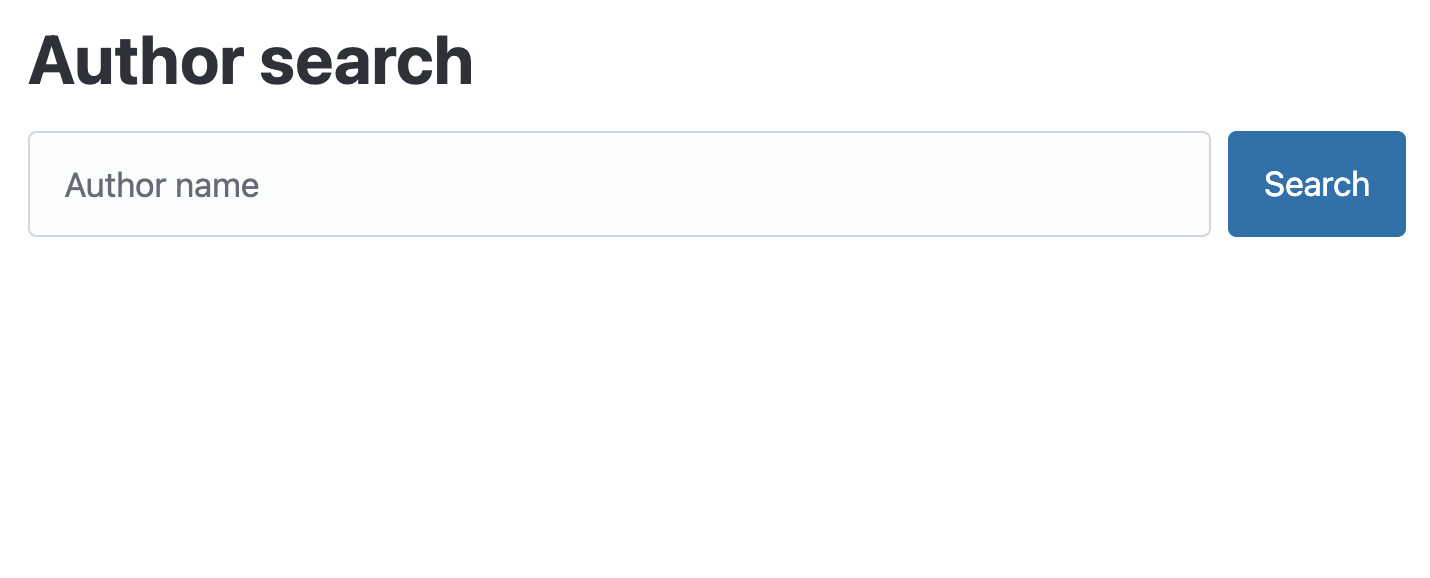
\includegraphics[scale=.4]{include/ui/search-form-1}
    \caption{Author search form}
    \label{fig:ui-search-form}
\end{figure}

\subsubsection{Search results} \label{sec:ui-results}

Figure~\ref{fig:ui-search-results} shows the search results page, displayed after the search form has been submitted, and the response has been returned.

Searching by name can return multiple results, matching the name, for each of the supported providers; the figure shows the list of results returned for ``skiadopoulos''.

\begin{figure}[tb]
    \centering
    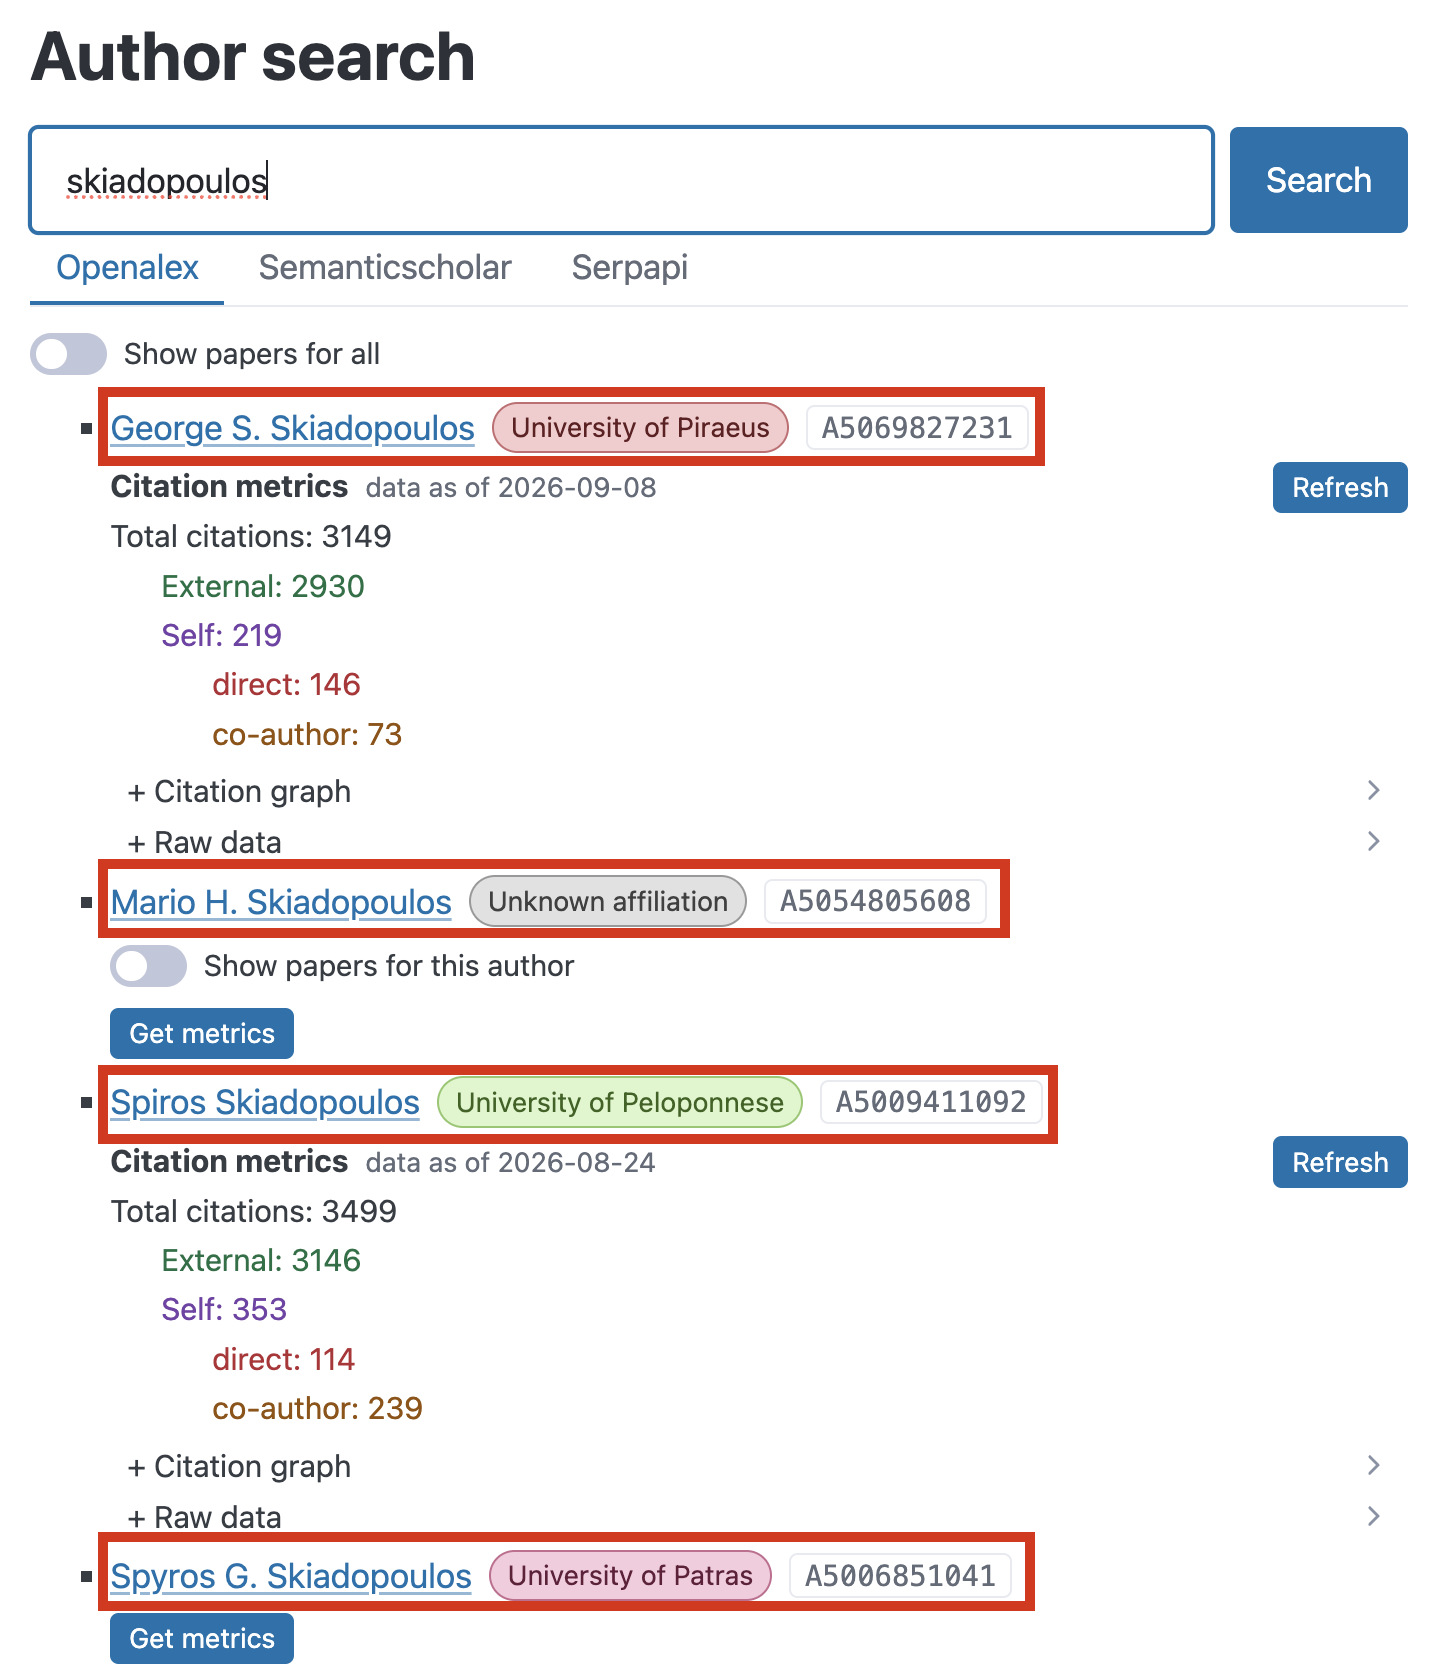
\includegraphics[scale=.4]{include/ui/search-res-1}
    \caption{Authors returned by one of the providers}
    \label{fig:ui-search-results}
\end{figure}

Each author name on the result list is accompanied by an affiliation, when available, and the identifier assigned by the selected provider.
The name is a link to the author detail page, described in Section~\ref{sec:ui-details}.

Figure~\ref{fig:ui-search-controls} shows the stored metrics, the update date and the refresh button of a profile.
The profiles, where results have not been collected previously, include a \emph{Get metrics} button, to request the citation counts.
For profiles, where citation metrics have previously been requested, and the citation graphs are found in the database, the UI shows the metrics and the date of the last update.
For these profiles there is a \emph{Refresh} button to request the data, ignoring the stored graph and cached responses.

\begin{figure}[tb]
    \centering
    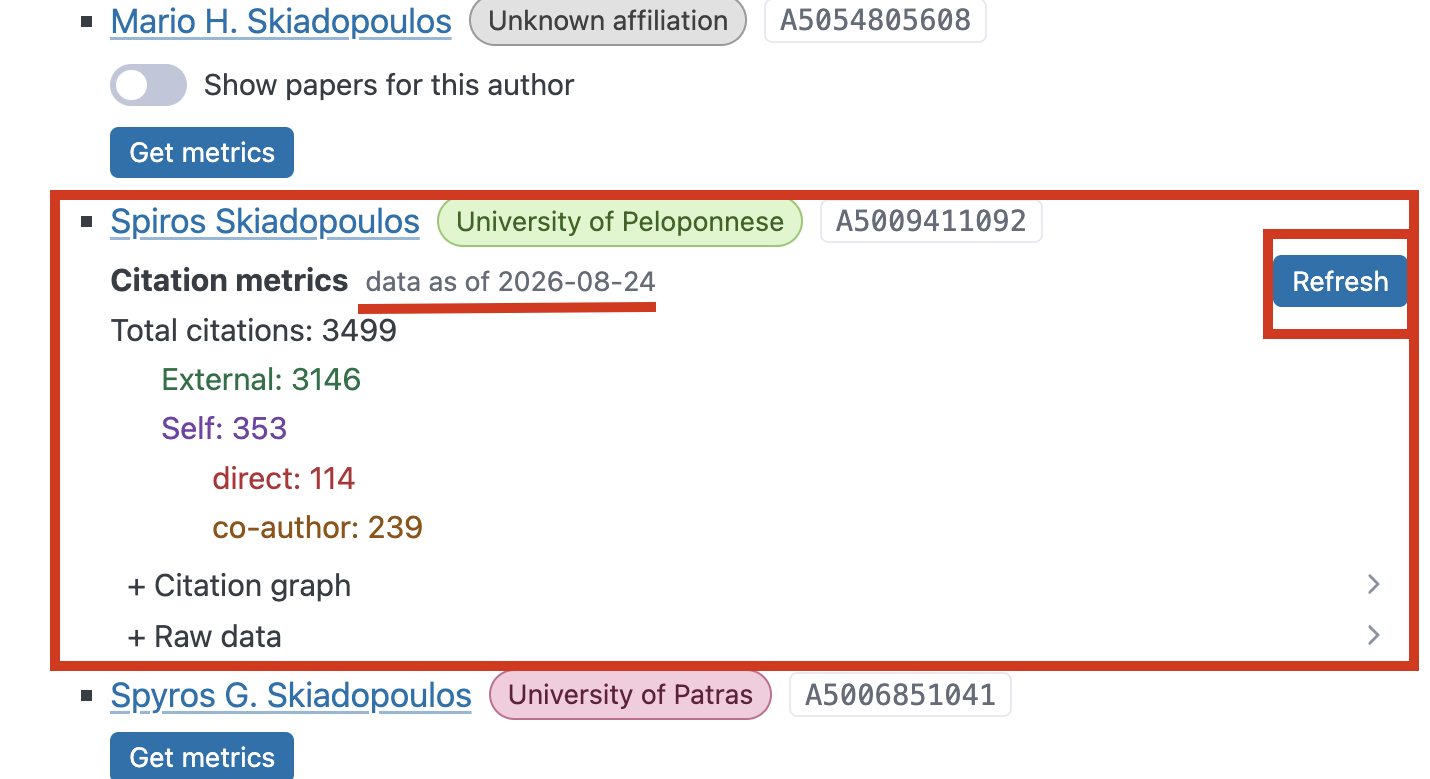
\includegraphics[scale=.4]{include/ui/search-res-2}
    \caption{Stored citation metrics, update date and refresh button}
    \label{fig:ui-search-controls}
\end{figure}

Figure~\ref{fig:ui-provider-tabs} highlights the selected provider.
The provider tabs keep results isolated per source, following the decision described in Section~\ref{sec:providers}.

\begin{figure}[tb]
    \centering
    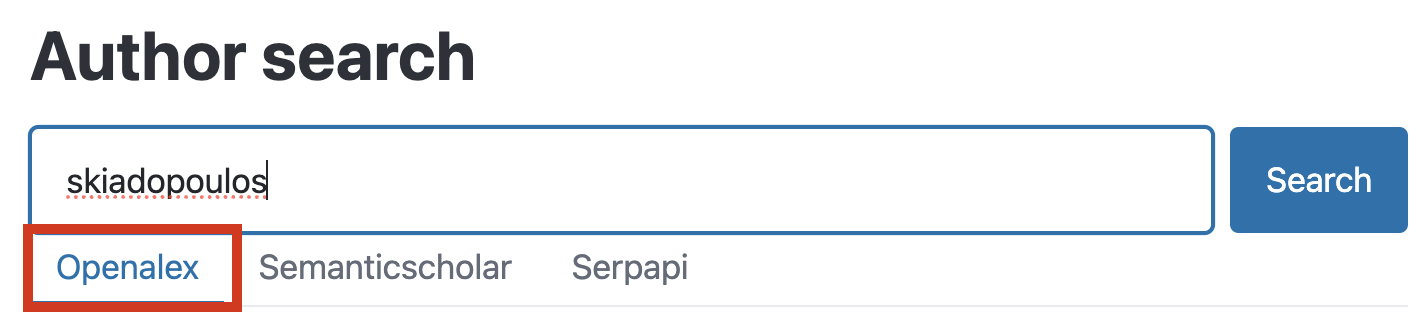
\includegraphics[scale=.4]{include/ui/search-res-4}
    \caption{Provider tabs in the search results}
    \label{fig:ui-provider-tabs}
\end{figure}

If search fails for a provider, its tab will display an error, not affecting the results of the other providers.

Figure~\ref{fig:ui-show-papers} shows the \emph{Show papers for all} switch, which applies to all the authors in the selected tab.
To help deterministically select the correct author, among ones with similar names and affiliations, the UI provides an option to display their publications.
A familiar title could be easier to recognize, especially if the author has changed affiliation, or shows no affiliation in the UI.

\begin{figure}[tb]
    \centering
    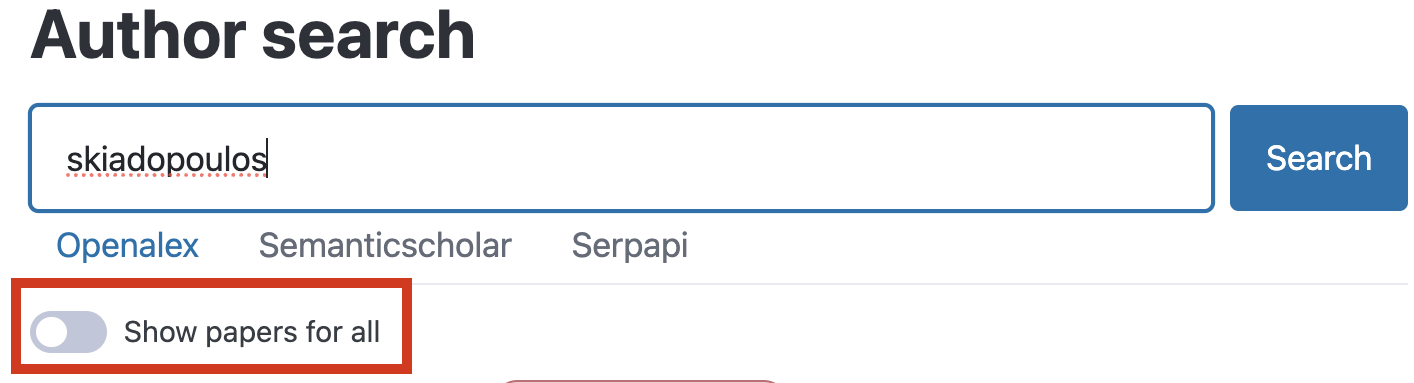
\includegraphics[scale=.4]{include/ui/search-res-5}
    \caption{Showing papers for all authors}
    \label{fig:ui-show-papers}
\end{figure}

Figure~\ref{fig:ui-unknown-affiliation} shows a profile without an affiliation, displayed as \emph{Unknown affiliation}: only such profiles include a switch to show the papers of the individual author.
This is helpful to avoid waiting for other authors on the list, and consuming the provider quotas.

\begin{figure}[tb]
    \centering
    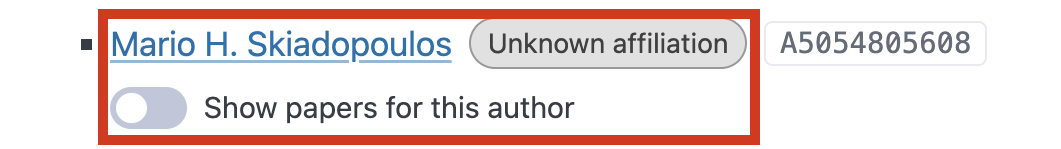
\includegraphics[scale=.4]{include/ui/search-res-3}
    \caption{An author without an affiliation}
    \label{fig:ui-unknown-affiliation}
\end{figure}

Figure~\ref{fig:ui-individual-papers} shows how the toggle to show the papers of an individual author alone works.

\begin{figure}[tb]
    \centering
    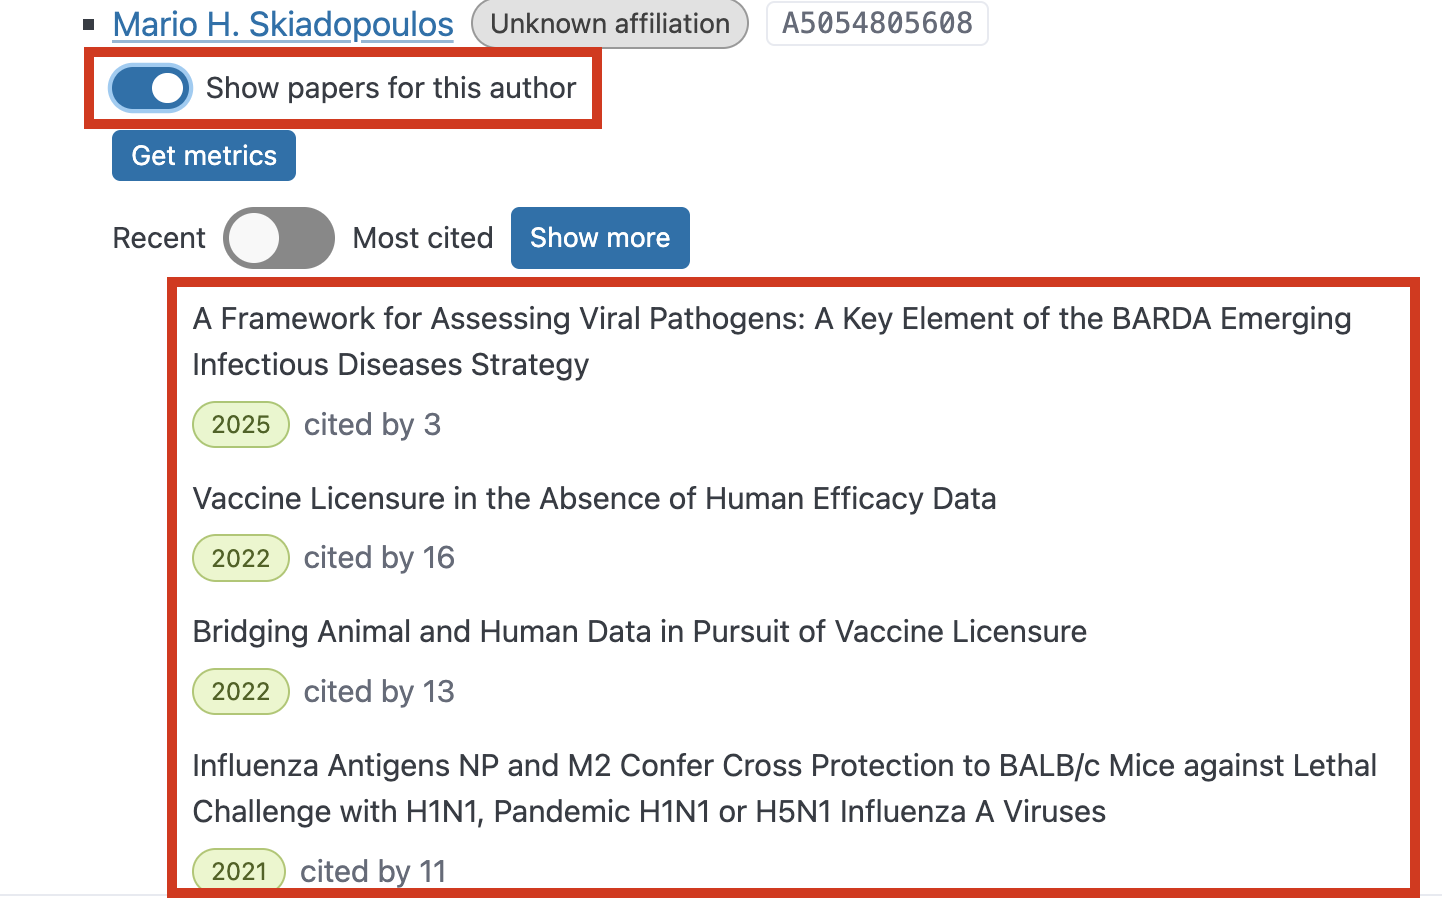
\includegraphics[scale=.4]{include/ui/search-res-5.3}
    \caption{Showing the papers of an author without an affiliation}
    \label{fig:ui-individual-papers}
\end{figure}

Figure~\ref{fig:ui-paper-order} shows the two ways of ordering the papers of the same author.
The list initially shows five papers, ordered by the publication date (\emph{most recent} first), with an option to order by citation count (\emph{most cited} first).
The \emph{Show more} button allows to load the rest of the list, beyond the initially shown five papers.

\begin{figure}[tb]
    \centering
    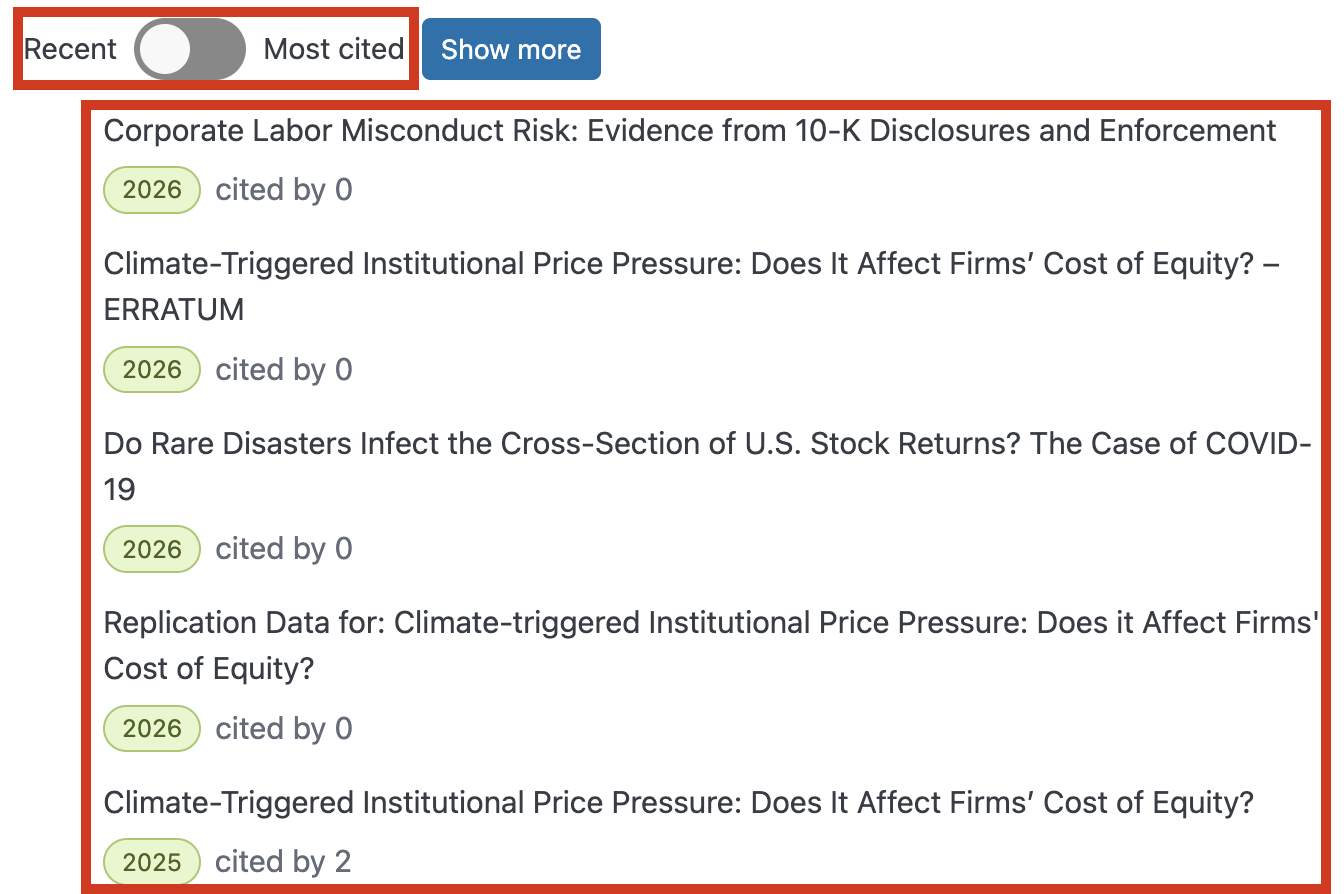
\includegraphics[scale=.3]{include/ui/search-res-5.1}
    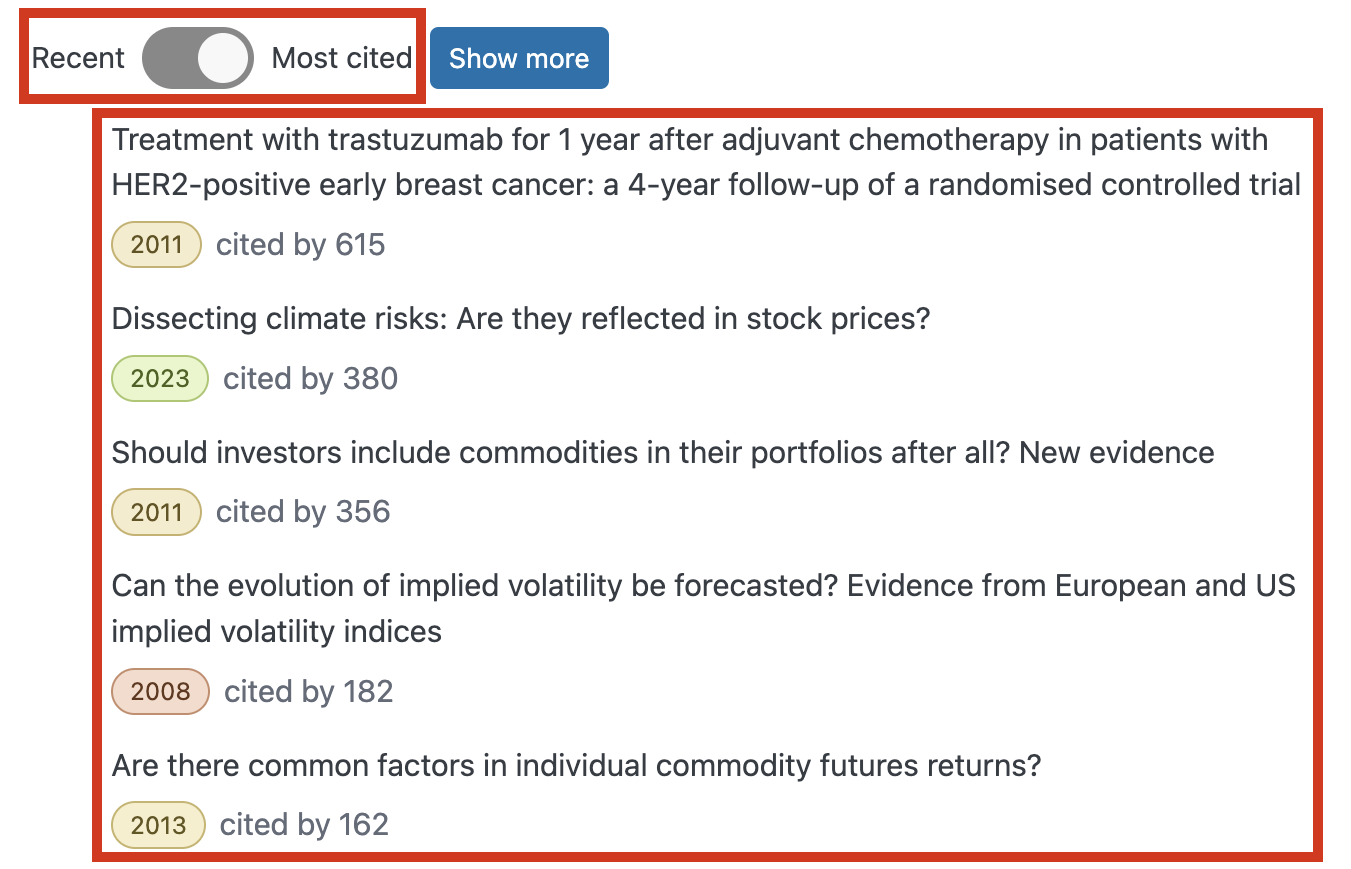
\includegraphics[scale=.3]{include/ui/search-res-5.2}
    \caption{Papers ordered most recent or most cited first}
    \label{fig:ui-paper-order}
\end{figure}

Users must explicitly request publication lists to be shown, to avoid unnecessary provider requests when the author is already recognizable.

Figure~\ref{fig:ui-get-metrics} shows the button \emph{Get metrics} that is available for every author, the user can click to request the citation metrics, starting the job as described in Section~\ref{sec:processing-pipeline}.

\begin{figure}[tb]
    \centering
    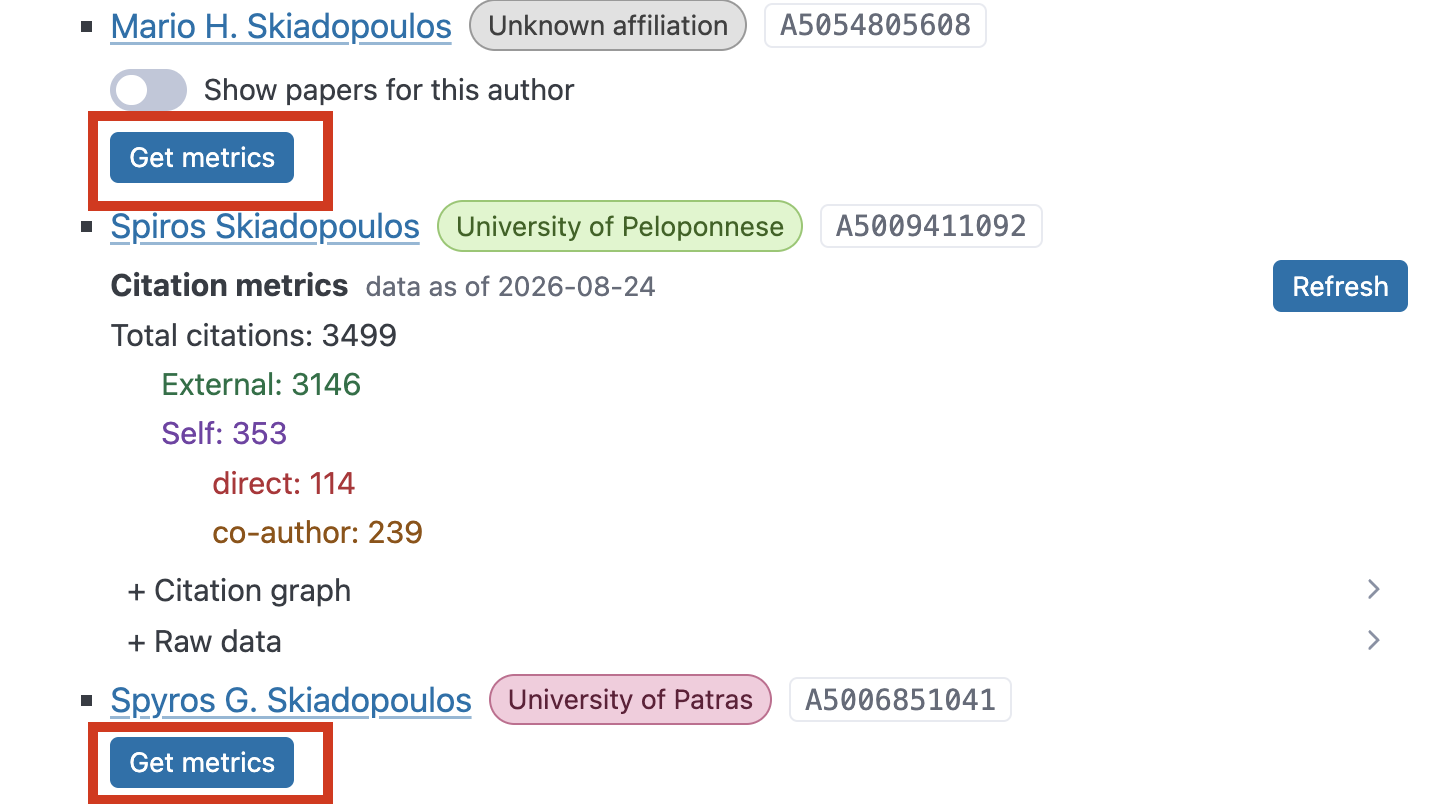
\includegraphics[scale=.4]{include/ui/search-res-6}
    \caption{Requesting citation metrics for an author}
    \label{fig:ui-get-metrics}
\end{figure}

Figure~\ref{fig:ui-metrics-progress} shows the progress under the selected author name, with the number of requests \textsf{completed}, \textsf{queued} and \textsf{failed}, updated while the job is running.

\begin{figure}[tb]
    \centering
    
\includegraphics[scale=.4]{include/ui/search-form-2}
    \caption{Progress while collecting the selected author's citations}
    \label{fig:ui-metrics-progress}
\end{figure}

Figure~\ref{fig:ui-metrics} shows the completed citation breakdown.
The completed result returns the breakdown of the number of citations, with counts for: \textsf{total}, \textsf{external}, and \textsf{direct} and \textsf{co-author} self-citations.

\begin{figure}[tb]
    \centering
    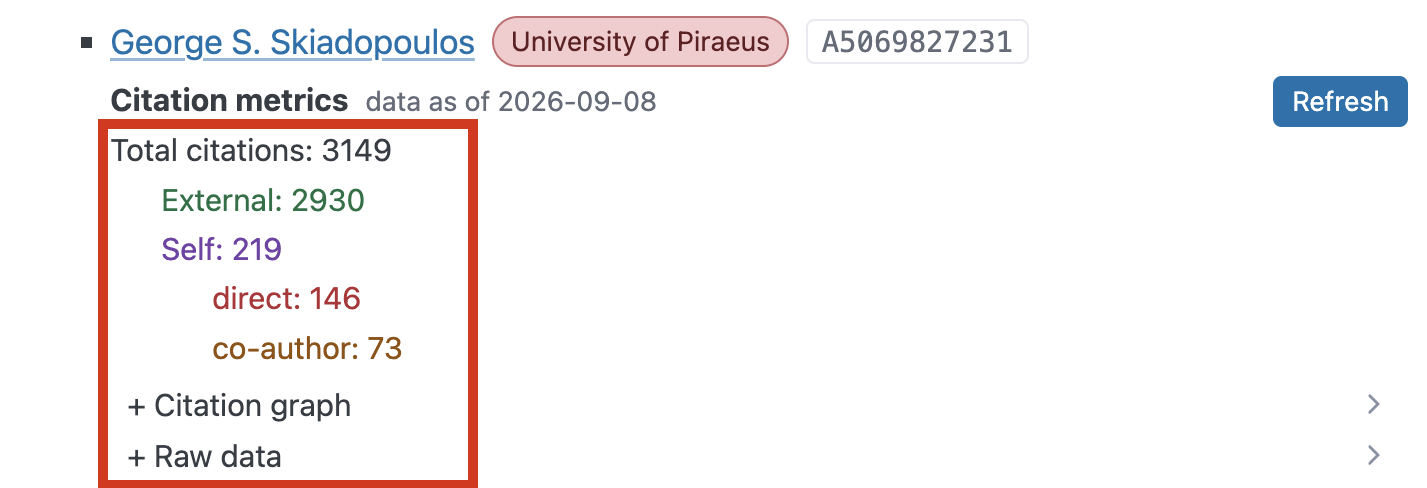
\includegraphics[scale=.4]{include/ui/search-res-7}
    \caption{The citation breakdown in the search results}
    \label{fig:ui-metrics}
\end{figure}

Counts summarize the result, but to provide more detailed information and a graph visualization, there are two initially collapsed options at the bottom of an author section.

Figure~\ref{fig:ui-graph} shows the graph chart, opened by clicking the \emph{Citation graph} link.
It represents the selected author, their own papers and the citing papers.

\begin{figure}[tb]
    \centering
    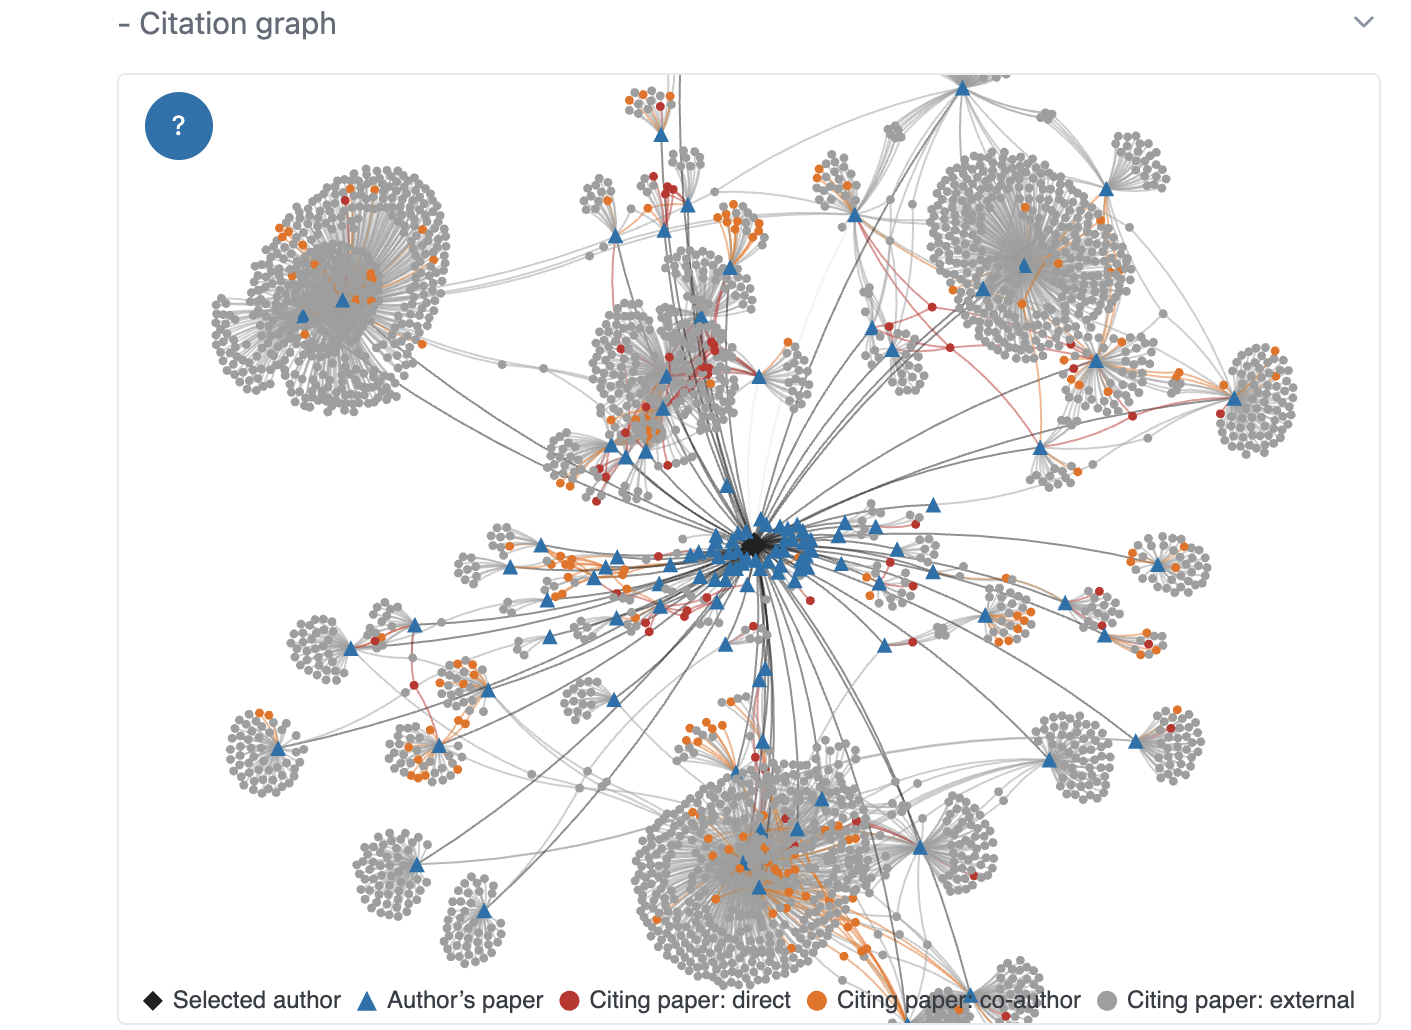
\includegraphics[scale=.4]{include/ui/author-details-2}
    \caption{The expanded citation graph}
    \label{fig:ui-graph}
\end{figure}

The connecting lines (graph edges) represent the relations between the selected author and their papers (\textsf{contribution}), and the selected author papers and citing papers (\textsf{citation}).

The graph supports zooming and panning, and hovering over a node reveals its details.

Figure~\ref{fig:ui-graph-filter} shows the graph filtered by excluding one of the node types.
There is a legend at the bottom of the chart explaining the shapes and colors of the graph, and acting as a filter, to hide or show the respective nodes by clicking on each category.
The citing papers are colored by the classification (\textsf{direct}, \textsf{co-author}, \textsf{external}).
A large graph is difficult to inspect with every citation visible; in the figure, the external citations are hidden, which leaves only the self-citations rendered in the graph.

\begin{figure}[tb]
    \centering
    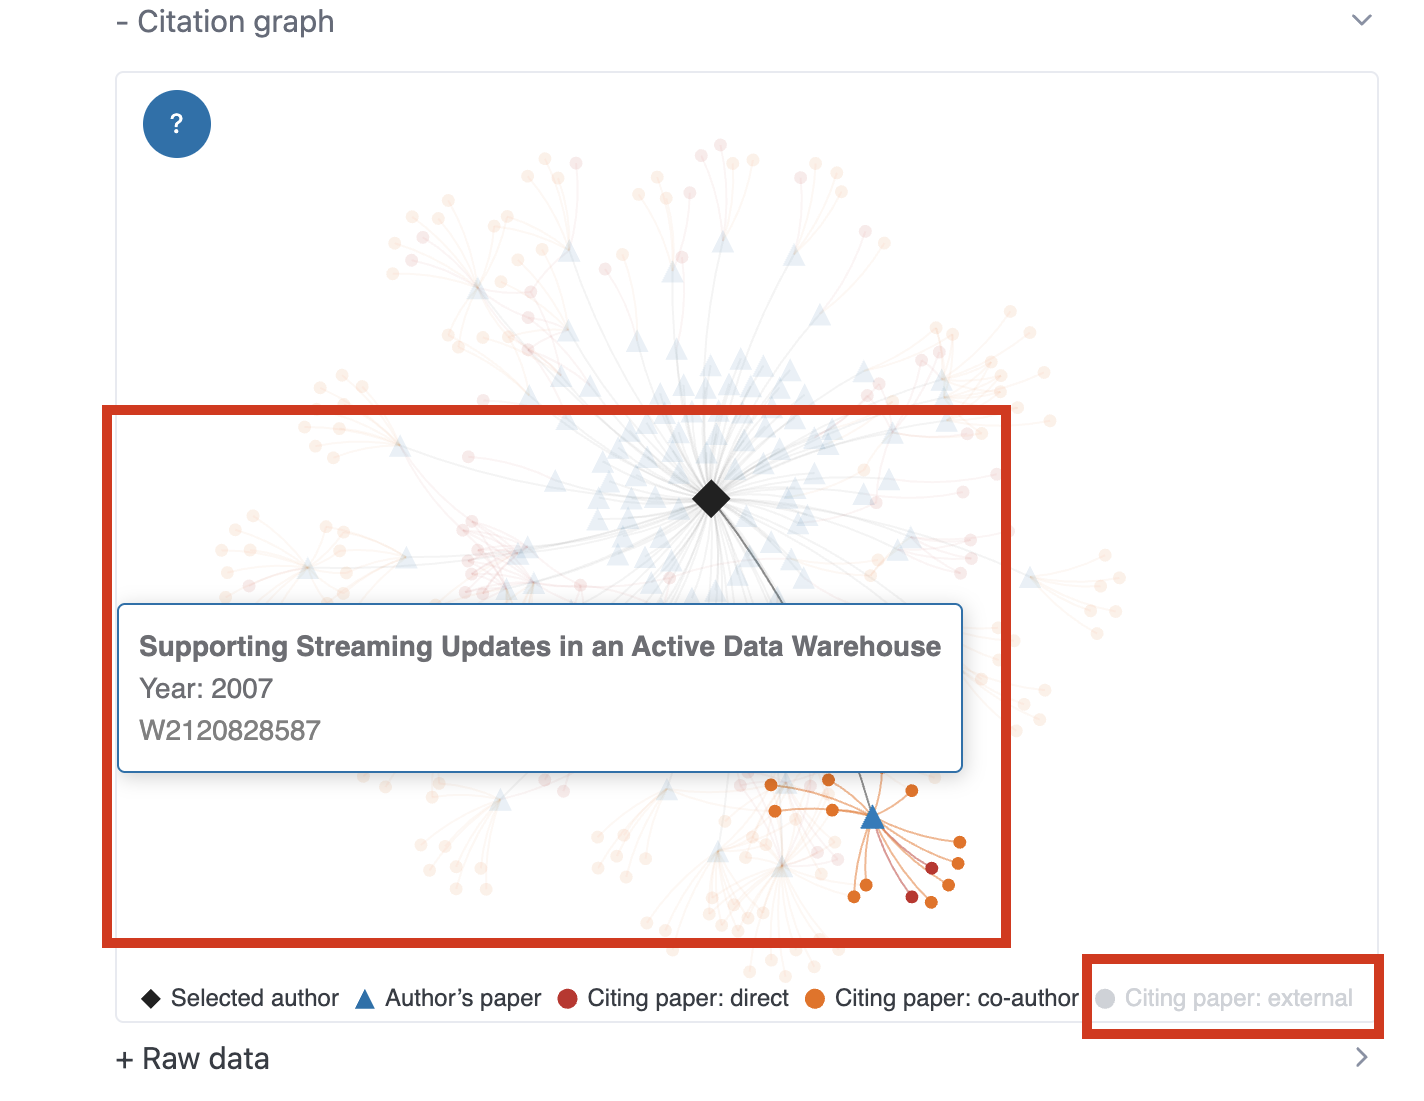
\includegraphics[scale=.4]{include/ui/author-details-5}
    \caption{Publication details with external citations hidden}
    \label{fig:ui-graph-filter}
\end{figure}

\subsubsection{Author details} \label{sec:ui-details}

\begin{figure}[tb]
    \centering
    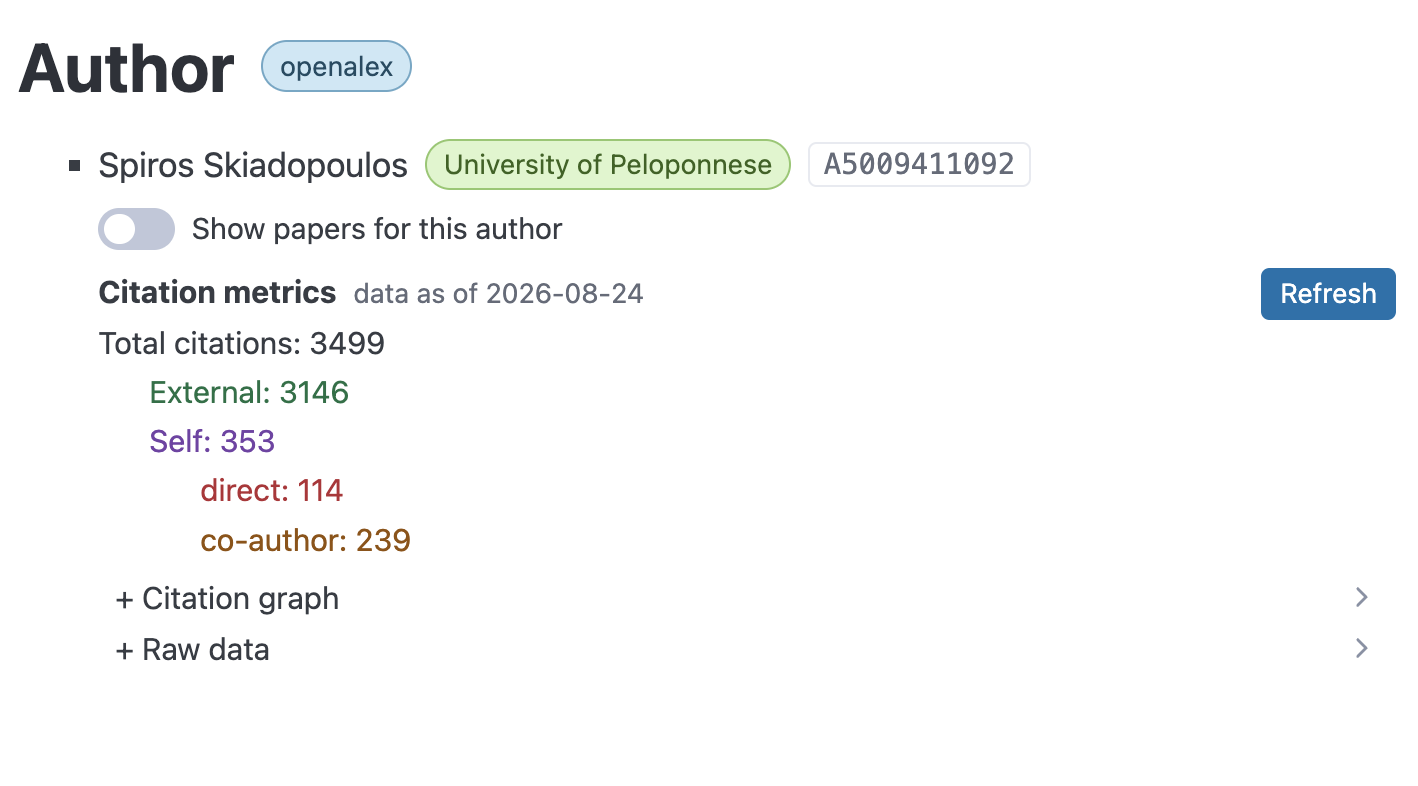
\includegraphics[scale=.4]{include/ui/author-details-1}
    \caption{A separate page for the selected author}
    \label{fig:ui-author}
\end{figure}

Figure~\ref{fig:ui-author} shows the page for the selected author, that can be opened by clicking on an author name.
As any other link, it can be opened in a new browser tab, allowing multiple author results to be open side by side.

The author name, the provider and the affiliation are rendered in the header of the page.
The remaining space on the page is occupied by the controls identical to the structure of the individual author details shown in the search results, as described in Section~\ref{sec:ui-results}.

\subsubsection{Status} \label{sec:ui-status}

Figure~\ref{fig:ui-status} shows the provider and system details panel.
Normally, it stays collapsed at the bottom of the page.
Clicking the \emph{Show status} button opens the panel, showing the request rate limit (requests per second), quotas, and the number of stored records for each provider, as well as jobs.
API keys are shown masked, only to identify that an API key is used, which can be helpful for providers that allow access with or without an API key, for instance \textsf{Semantic Scholar}.

The application version, together with the system resources (including the available memory and disk space) appear below the table.
These details are useful when investigating service disruptions.

\begin{figure}[tb]
    \centering
    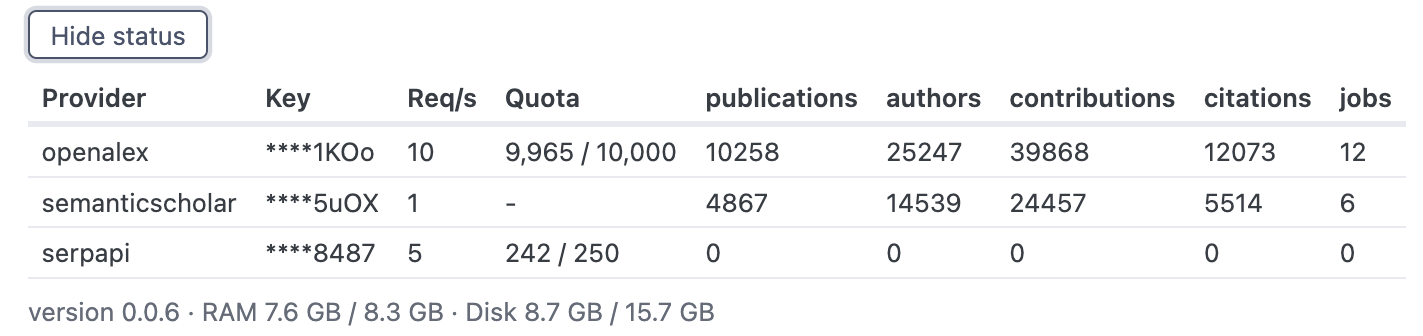
\includegraphics[scale=.4]{include/ui/status-1}
    \caption{Provider and system status}
    \label{fig:ui-status}
\end{figure}

\subsection{Testing} \label{sec:testing}

The backend, as the subsystem containing all business logic, is covered by automated tests, validating the outputs of all units of each component in isolation (such as services, repositories, connectors, controllers).
The unit tests guarantee that the behavior of each unit remains within the expectations.

The tests are written with \textsf{Jest}\footnote{\url{https://jestjs.io}} - one of the popular JavaScript unit test libraries.
Tests are organized into suites, where each suite covers the behavior of a single component.

The tests never touch real databases, the clock or the network.
Instead, every dependency of the unit under test is replaced by a mock fixture, allowing to program the expected results on each invocation.

This approach is convenient to make the unsuccessful paths reproducible.
By mocking the dependencies, unit tests can simulate all paths of behavior of an external provider: successful or erroneous responses, malformed data, empty results and so on.

The tests are placed near the components they cover, in \textsf{\_\_tests\_\_} directories at the same file system level.

On every push to the repository, a workflow executed by a \textsf{GitHub Actions} runner invokes the unit tests, and if any one of these fails, the pipeline exits with an error.
This mechanism prevents building and deploying versions of the application with invalid logic.

The unit tests follow a convenient nested structure, allowing to cover every branch of the source code logic.
Each level explores a scenario, by progressively refining the circumstances, to finally get to the inner blocks starting with \emph{it}, which performs a single call and asserts an outcome expectation.

Listing~\ref{lst:retry-tests} shows the outlined version of the suite testing \textsf{RetryStrategy}, the component responsible for retrying failed requests.
The method \textsf{run} executes the target function, and if the outcome is deemed retriable, it repeats the call, to either reach a successful outcome or exhaust the maximum allowed number of retries.

\begin{lstlisting}[float=tb, language=Java, caption={Structure of the retry strategy unit test suite}, label={lst:retry-tests}]
describe('RetryStrategy', () => {
  describe('run', () => {
    describe('when the function succeeds', () => {
      it('returns the value', ...);
      it('calls the function once', ...);
    });
    describe('when the function fails', () => {
      describe('but the error is not retryable', () => {
        it('does not retry', ...);
        it('passes the error to the retry check', ...);
      });
      describe('and the error is retryable', () => {
        describe('and a retry succeeds', () => {
          it('returns the eventual value', ...);
          it('stops calling once it succeeds', ...);
        });
        describe('but the retries are exhausted', () => {
          it('gives up with the error', ...);
          it('tries maxRetries + 1 times', ...);
        });
      });
    });
  });
});
\end{lstlisting}

Running the suite prints the titles of each branch and test, resulting in the same nested structure.
Listing~\ref{lst:retry-test-run} shows the output of the same retry strategy suite.

\begin{lstlisting}[float=tb, caption={Output of the retry strategy unit tests}, label={lst:retry-test-run}, literate={✓}{{\ensuremath\checkmark}}1]
PASS src/lib/__tests__/RetryStrategy.test.js
  RetryStrategy
    run
      when the function succeeds
        ✓ returns the value
        ✓ calls the function once
      when the function fails
        but the error is not retryable
          ✓ does not retry
          ✓ passes the error to the retry check
        and the error is retryable
          and a retry succeeds
            ✓ returns the eventual value
            ✓ stops calling once it succeeds
          but the retries are exhausted
            ✓ gives up with the error
            ✓ tries maxRetries + 1 times

\end{lstlisting}

\section{Evaluation} \label{sec:evaluation}

This section evaluates the results produced by the system: given an author, return the counts of their total citations by contribution category.
Each author represents an atomic use case, where the entirety of their publications is considered at the time of evaluation.
Section~\ref{sec:classification-checks} evaluates the classification algorithm in isolation, by comparing the output of the respective function to manually counted citations for a single use case.
Section~\ref{sec:data-source-comparison} compares the data and results of the same author, retrieved from different providers.

\subsection{Citation classification} \label{sec:classification-checks}

To evaluate the work of the citation classification function, let us consider an author, for instance \emph{Spiros Skiadopoulos}.
Following the implemented methodology, described in Section~\ref{sec:processing-pipeline}, the evaluation is carried out in the context of a single provider, for instance \emph{OpenAlex}.

The classification function compares the authors of each cited and citing publication, to calculate the citation classification as \emph{direct}, \emph{co-author} or \emph{external}.

To operate on realistic data, we have retrieved all records from the selected provider for the selected author on 9 October 2026, and stored a normalized citation graph in the local database.
Going forward, to analyze data, we will be using SQL queries and their results; this will help make the evaluation framework clear to understand and reproducible.

Tables~\ref{tab:sample-publications}--\ref{tab:sample-citations} demonstrate a sample of records in the tables of the local database.


\begin{table}[tb]
    \centering
    \begin{tabular}{|l|l|}
        \hline
        Field & Value \\
        \hline\hline
        provider & openalex \\
        pub\_id & W3141363959 \\
        title & inTIME: A Machine Learning-Based Framework for \dots \\
        normalised\_title & intime: a machine learning-based framework for \dots \\
        external\_id & https://doi.org/10.3390/electronics10070818 \\
        year & 2021 \\
        citation\_count & \\
        \hline
    \end{tabular}
    \caption{A sample record of the \texttt{publications} table}
    \label{tab:sample-publications}
\end{table}

\begin{table}[tb]
    \centering
    \footnotesize
    \begin{tabular}{|l|l|l|l|l|}
        \hline
        provider & author\_id & original\_name & normalised\_name & organisation \\
        \hline\hline
        openalex & A5046481193 & Paris Koloveas & paris koloveas & University of Peloponnese \\
        openalex & A5054180455 & Thanasis Chantzios & thanasis chantzios & University of Peloponnese \\
        \hline
    \end{tabular}
    \caption{Sample records of the \texttt{authors} table}
    \label{tab:sample-authors}
\end{table}

\begin{table}[tb]
    \centering
    \begin{tabular}{|l|l|l|r|}
        \hline
        provider & pub\_id & author\_id & position \\
        \hline\hline
        openalex & W3141363959 & A5046481193 & 1 \\
        openalex & W3141363959 & A5054180455 & 2 \\
        \hline
    \end{tabular}
    \caption{Sample records of the \texttt{contributions} table}
    \label{tab:sample-contributions}
\end{table}

\begin{table}[tb]
    \centering
    \begin{tabular}{|l|l|l|}
        \hline
        provider & source\_pub\_id & target\_pub\_id \\
        \hline\hline
        openalex & W4386028955 & W3141363959 \\
        openalex & W4200158199 & W3141363959 \\
        \hline
    \end{tabular}
    \caption{Sample records of the \texttt{citations} table}
    \label{tab:sample-citations}
\end{table}

Each of the steps below defines a named query, building on the previously defined named queries.
The complete query is built at the end, combining all the steps and producing the final result.

The selected author is found in the \texttt{authors} table.

\begin{quote}
    \begin{vercode}
WITH selected_author AS (
    SELECT *
    FROM authors
    WHERE provider = 'openalex'
        AND normalised_name = 'spiros skiadopoulos'
)
    \end{vercode}
\end{quote}

\begin{center}
    \begin{tabular}{|l|l|}
        \hline
        Column & Value \\
        \hline\hline
        provider & openalex \\
        author\_id & A5009411092 \\
        original\_name & Spiros Skiadopoulos \\
        normalised\_name & spiros skiadopoulos \\
        organisation & University of Peloponnese \\
        \hline
    \end{tabular}
\end{center}

The selected author has multiple records in the \texttt{contributions} table.

\begin{quote}
    \begin{vercode}
WITH author_contributions AS (
    SELECT c.*
    FROM contributions c
        JOIN selected_author sa
            ON c.provider = sa.provider
                AND c.author_id = sa.author_id
)
    \end{vercode}
\end{quote}

\begin{center}
    \begin{tabular}{|l|l|l|r|}
        \hline
        provider & pub\_id & author\_id & position \\
        \hline\hline
        openalex & W129833210 & A5009411092 & 3 \\
        openalex & W141810174 & A5009411092 & 3 \\
        \multicolumn{4}{|c|}{$\vdots$} \\
        \multicolumn{4}{|c|}{Total: 117 records} \\
        \hline
    \end{tabular}
\end{center}

The selected author's publication citations are stored in the \texttt{citations} table.
The column \texttt{target\_pub\_id} indicates that these are all incoming citations.

\begin{quote}
    \begin{vercode}
WITH author_citations AS (
    SELECT ci.*
    FROM citations ci
        JOIN author_contributions ac
            ON ci.provider = ac.provider
                AND ci.target_pub_id = ac.pub_id
)
    \end{vercode}
\end{quote}

\begin{center}
    \begin{tabular}{|r|}
        \hline
        num\_citations\_total \\
        \hline\hline
        3584 \\
        \hline
    \end{tabular}
\end{center}

We select \emph{direct} citations from all author citations by matching the author contributions with the \texttt{source\_pub\_id} of the author citations.

\begin{quote}
    \begin{vercode}
WITH direct_citations AS (
    SELECT aci.*
    FROM author_citations aci
        JOIN author_contributions ac
            ON aci.provider = ac.provider
                AND aci.source_pub_id = ac.pub_id
)
    \end{vercode}
\end{quote}

\begin{center}
    \begin{tabular}{|r|}
        \hline
        num\_citations\_direct \\
        \hline\hline
        115 \\
        \hline
    \end{tabular}
\end{center}

The remaining citations, where the selected author is not an author of a citing publication, are either \emph{co-author} or \emph{external} citations.

\begin{quote}
    \begin{vercode}
WITH indirect_citations AS (
    SELECT aci.*
    FROM author_citations aci
        LEFT OUTER JOIN direct_citations dc
            ON aci.provider = dc.provider
                AND aci.source_pub_id = dc.source_pub_id
                AND aci.target_pub_id = dc.target_pub_id
    WHERE dc.source_pub_id IS NULL
)
    \end{vercode}
\end{quote}

\begin{center}
    \begin{tabular}{|r|}
        \hline
        num\_citations\_indirect \\
        \hline\hline
        3469 \\
        \hline
    \end{tabular}
\end{center}

The \emph{co-author} citations are those where the selected author is not an author of a citing publication, but the citing and cited publications share at least one other author.

\begin{quote}
    \begin{vercode}
WITH coauthor_citations AS (
    SELECT DISTINCT ic.*
    FROM indirect_citations ic
        JOIN contributions cited
            ON cited.provider = ic.provider
                AND cited.pub_id = ic.target_pub_id
        JOIN contributions citing
            ON citing.provider = ic.provider
                AND citing.pub_id = ic.source_pub_id
                AND citing.author_id = cited.author_id
)
    \end{vercode}
\end{quote}

\begin{center}
    \begin{tabular}{|r|}
        \hline
        num\_citations\_coauthor \\
        \hline\hline
        243 \\
        \hline
    \end{tabular}
\end{center}

The \emph{external} citations are those where the citing and cited publications share no author at all.

\begin{quote}
    \begin{vercode}
WITH external_citations AS (
    SELECT ic.*
    FROM indirect_citations ic
        LEFT OUTER JOIN coauthor_citations cc
            ON ic.provider = cc.provider
                AND ic.source_pub_id = cc.source_pub_id
                AND ic.target_pub_id = cc.target_pub_id
    WHERE cc.source_pub_id IS NULL
)
    \end{vercode}
\end{quote}

\begin{center}
    \begin{tabular}{|r|}
        \hline
        num\_citations\_external \\
        \hline\hline
        3226 \\
        \hline
    \end{tabular}
\end{center}

The complete query combines all the steps above and returns all the counts at once.

\begin{quote}
    \begin{vercode}
WITH
selected_author AS (
    SELECT *
    FROM authors
    WHERE provider = 'openalex'
        AND normalised_name = 'spiros skiadopoulos'
),
author_contributions AS (
    SELECT c.*
    FROM contributions c
        JOIN selected_author sa
            ON c.provider = sa.provider
                AND c.author_id = sa.author_id
),
author_citations AS (
    SELECT ci.*
    FROM citations ci
        JOIN author_contributions ac
            ON ci.provider = ac.provider
                AND ci.target_pub_id = ac.pub_id
),
direct_citations AS (
    SELECT aci.*
    FROM author_citations aci
        JOIN author_contributions ac
            ON aci.provider = ac.provider
                AND aci.source_pub_id = ac.pub_id
),
indirect_citations AS (
    SELECT aci.*
    FROM author_citations aci
        LEFT OUTER JOIN direct_citations dc
            ON aci.provider = dc.provider
                AND aci.source_pub_id = dc.source_pub_id
                AND aci.target_pub_id = dc.target_pub_id
    WHERE dc.source_pub_id IS NULL
),
coauthor_citations AS (
    SELECT DISTINCT ic.*
    FROM indirect_citations ic
        JOIN contributions cited
            ON cited.provider = ic.provider
                AND cited.pub_id = ic.target_pub_id
        JOIN contributions citing
            ON citing.provider = ic.provider
                AND citing.pub_id = ic.source_pub_id
                AND citing.author_id = cited.author_id
),
external_citations AS (
    SELECT ic.*
    FROM indirect_citations ic
        LEFT OUTER JOIN coauthor_citations cc
            ON ic.provider = cc.provider
                AND ic.source_pub_id = cc.source_pub_id
                AND ic.target_pub_id = cc.target_pub_id
    WHERE cc.source_pub_id IS NULL
)
SELECT
    (SELECT COUNT(*) FROM author_citations)
        AS num_citations_total,
    (SELECT COUNT(*) FROM direct_citations)
        AS num_citations_direct,
    (SELECT COUNT(*) FROM coauthor_citations)
        AS num_citations_coauthor,
    (SELECT COUNT(*) FROM external_citations)
        AS num_citations_external;
    \end{vercode}
\end{quote}

\begin{center}
    \begin{tabular}{|r|r|r|r|}
        \hline
        total & direct & co-author & external \\
        \hline\hline
        3584 & 115 & 243 & 3226 \\
        \hline
    \end{tabular}
\end{center}

Figure~\ref{fig:sample-counts} shows the counts calculated by the system for the same author and provider.
The three subtotals produce the expected total ($115 + 243 + 3226 = 3584$), matching the system counts.

\begin{figure}[tb]
    \centering
    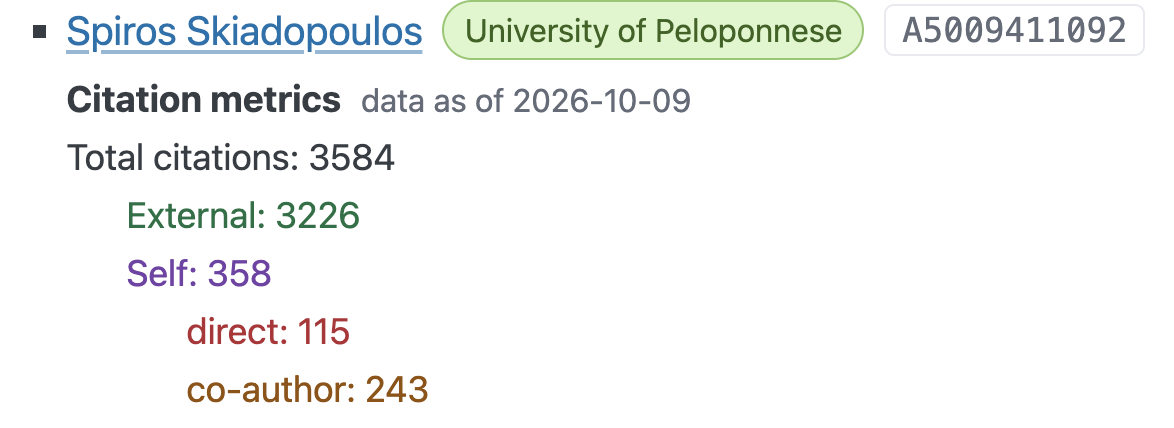
\includegraphics[scale=.4]{include/fig-sample-counts}
    \caption{Sample counts calculated by the system}
    \label{fig:sample-counts}
\end{figure}

\subsection{Comparison of data sources} \label{sec:data-source-comparison}

To evaluate and compare the data sources, we used a sample of one author and searched the same author with each of the providers.
The identifiers below represent the same author, \emph{Spiros Skiadopoulos}, as returned from different providers: \texttt{A5009411092} from \textsf{OpenAlex}, \texttt{1688897} from \textsf{Semantic Scholar} and \texttt{fxBHpbgAAAAJ} from \textsf{Google Scholar}.
All data were updated on the same date, 10 October 2026.

None of the provider data or the produced counts match precisely.

Table~\ref{tab:provider-distribution} illustrates the distribution of the publications of the selected author across the providers.
As each provider exposes their own publication identifier, and in an attempt to compare the papers returned by each source, we compared publications by normalized title, and discovered that there are 236 distinct titles for the same author in total, where only 71 match across all providers.

\begin{table}[tb]
    \centering
    \begin{minipage}[c]{0.6\linewidth}
        \centering
        \small
        \begin{tabular}{|l|r|}
            \hline
            Publications (by normalized\_title) & Count \\
            \hline\hline
            on any provider (union) & 236 \\
            on all providers (intersection) & 71 \\
            exclusive to \textsf{OpenAlex} & 12 \\
            exclusive to \textsf{Semantic Scholar} & 101 \\
            exclusive to \textsf{Google Scholar} & 32 \\
            \hline
        \end{tabular}
    \end{minipage}

    \medskip
    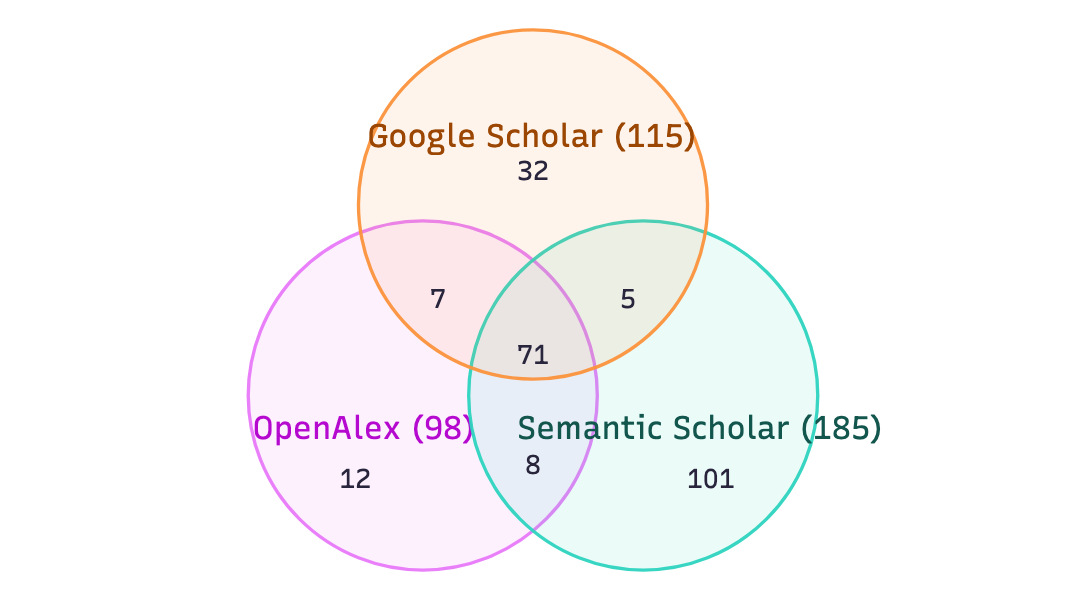
\includegraphics[scale=.2]{include/fig-provider-distribution-diagram}
    \caption{Distribution of author publications by source}
    \label{tab:provider-distribution}
\end{table}

Table~\ref{tab:provider-comparison} contains the publication and citation counts, per provider.

\begin{table}[tb]
    \centering
    \footnotesize
    \setlength{\tabcolsep}{3pt}
    \begin{tabular}{|l|r|r|r|r|r|r|r|r|}
        \hline
        Provider & \shortstack{Publi-\\cations} & \shortstack{With\\citations} & \shortstack{Without\\citations} & Citations & \shortstack{Self-\\citations} & Direct & Co-author & External \\
        \hline\hline
        \textsf{OpenAlex} & 117 & 85 & 32 & 3584 & \shortstack[r]{358\\(10.0\%)} & \shortstack[r]{115\\(3.2\%)} & \shortstack[r]{243\\(6.8\%)} & \shortstack[r]{3226\\(90.0\%)} \\
        \textsf{Semantic Scholar} & 187 & 104 & 83 & 4093 & \shortstack[r]{351\\(8.6\%)} & \shortstack[r]{96\\(2.3\%)} & \shortstack[r]{255\\(6.2\%)} & \shortstack[r]{3742\\(91.4\%)} \\
        \textsf{Google Scholar} & 157 & 86 & 71 & 5458 & \shortstack[r]{76\\(1.4\%)} & \shortstack[r]{76\\(1.4\%)} & \shortstack[r]{0\\(0.0\%)} & \shortstack[r]{5382\\(98.6\%)} \\
        \hline
    \end{tabular}
    \caption{Publication and citation counts for \emph{Spiros Skiadopoulos}, by provider}
    \label{tab:provider-comparison}
\end{table}

All three providers include papers for which no citations were found: 32/117 in \textsf{OpenAlex}, 83/187 in \textsf{Semantic Scholar} and 71/157 in \textsf{Google Scholar} (mainly these are duplicates and alternative versions of cited papers)..
The most cited papers of the selected author are ``Conceptual modeling for ETL processes'' and ``PRIVE: anonymous location-based queries in distributed mobile systems'', across all sources.

In broad terms, the \textsf{OpenAlex} and \textsf{Semantic Scholar} numbers are the closest.
\textsf{Semantic Scholar} returned more papers and more citations than \textsf{OpenAlex} in absolute numbers, but the proportions are similar, as shown in Table~\ref{tab:provider-comparison}.
At the same time, \textsf{Google Scholar} returned more citations than the other two, though very few were classified as self-citations ($<$\,2\%), and all of them as \textsf{direct}.

\textsf{OpenAlex} and \textsf{Semantic Scholar} produced the same classification for 1798/1811 (99\%) citations, including all 57 \textsf{direct}.
The remaining 13 citations alternate between \textsf{co-author} and \textsf{external}, depending on the way providers resolve citing authors.

\textsf{Google Scholar} numbers stand out and seem misleading, compared to either of the other two providers, where author identities are available.

\begin{description}
    \item [Compared to \textsf{OpenAlex}] all citations classified as \textsf{co-author}, and almost half (29/65) of those classified as \textsf{direct}, are \textsf{external} in \textsf{Google Scholar}.
    \item [Compared to \textsf{Semantic Scholar}] almost all (165/167) \textsf{co-author} citations, and almost half (25/57) \textsf{direct} ones, are \textsf{external} in \textsf{Google Scholar}.
\end{description}

For \textsf{Google Scholar} the classification relies on matching authors by plain text names, as described in Section~\ref{sec:data}.
This results in citations classified as \textsf{direct} when the selected author is on the citing publication; otherwise the citation is classified as \textsf{external}.
The citing papers do not always include the profile identifier, resulting in even fewer matches for \textsf{direct}.

The following examples demonstrate the differences.

The first example is the citation discussed in Chapter~\ref{c1:intro}, where {[KGMP2007]}~\cite{Kalnis2007} cites {[GPK2007]}~\cite{Ghinita2007}.
\textsf{OpenAlex} and \textsf{Semantic Scholar} return author identities for both papers, so for Spiros Skiadopoulos the citation is classified as \textsf{co-author}.
For \textsf{Google Scholar} data, the same citation is classified as \textsf{external}.
Listing~\ref{lst:example-coauthor} shows the parsed data from the responses.

\begin{lstlisting}[float=tb, basicstyle=\footnotesize\ttfamily, caption={Authors of {[GPK2007]} and {[KGMP2007]}, as returned by providers}, label={lst:example-coauthor}]
// OpenAlex - [GPK2007]
[["A5069236544", "Gabriel Ghinita"], ["A5014399734", "Panos Kalnis"],
 ["A5009411092", "Spiros Skiadopoulos"]]
// OpenAlex - [KGMP2007]
[["A5014399734", "Panos Kalnis"], ["A5069236544", "Gabriel Ghinita"],
 ["A5053720072", "Kyriakos Mouratidis"], ["A5091887420", "Dimitris Papadias"]]

// Semantic Scholar - [GPK2007]
[{"authorId": "2182067502", "name": "G. Ghinita"},
 {"authorId": "2000187", "name": "Panos Kalnis"},
 {"authorId": "1688897", "name": "S. Skiadopoulos"}]
// Semantic Scholar - [KGMP2007]
[{"authorId": "2000187", "name": "Panos Kalnis"},
 {"authorId": "2182067502", "name": "G. Ghinita"},
 {"authorId": "1753946", "name": "K. Mouratidis"},
 {"authorId": "1746338", "name": "Dimitris Papadias"}]

// Google Scholar - [GPK2007]
"authors": "G Ghinita, P Kalnis, S Skiadopoulos"
// Google Scholar - [KGMP2007]
[{"name": "P Kalnis", "author_id": "-NdSrrYAAAAJ"},
 {"name": "G Ghinita", "author_id": "t_AzcmUAAAAJ"},
 {"name": "K Mouratidis", "author_id": "vq5oTnEAAAAJ"}]
\end{lstlisting}

The second example demonstrates provider errors resulting in skewed citation counts.
\textsf{OpenAlex} returns the paper {[Terrovitis2004]}~\cite{Terrovitis2004} as citing itself, which counts as a \textsf{direct} citation.
At the same time, \textsf{Google Scholar} returns ``S Skiadopoulost'' as an author for the same work, with nothing else matching this name, and the name matching no profile.
Listing~\ref{lst:example-errors} includes both records.

\begin{lstlisting}[float=tb, basicstyle=\footnotesize\ttfamily, caption={Errors in the responses of \textsf{OpenAlex} and \textsf{Google Scholar}}, label={lst:example-errors}]
// OpenAlex
{"id": "https://openalex.org/W4241330289",
 "title": "Modeling and language support for the management of pattern-bases",
 "publication_year": 2004,
 "referenced_works": [..., "https://openalex.org/W4241330289", ...]}

// Google Scholar
{"result_id": "WY_w50sssDEJ",
 "title": "Modeling and Language Support for the Management of",
 "publication_info": {
   "summary": "S Skiadopoulost, E Bertinos - International Conference on ..., 2004",
   "authors": [{"name": "S Skiadopoulost"}, {"name": "E Bertinos"}]}}
\end{lstlisting}

Having analyzed one sample author, we have shown that the data returned by each provider does not overlap precisely with data returned by other providers.
Also, we have demonstrated that none of the sources used in this work was 100\% accurate and curated.
The accuracy of classification counts, derived from inaccurate data, are still a good statisticall approach, though should be treated with care.

% !TEX encoding = UTF-8 Unicode
% !TEX root = thesis-main.tex

\chapterr{Συμπεράσματα και μελλοντικές επεκτάσεις}
Στο προηγούμενο κεφάλαιο παρουσιάσαμε σχετικά συστήματα και ερευνητικές εργασίες που μας βοήθησαν στην ανάλυση των απαιτήσεων του \textlatin{MeL}.  Σε αυτό το κεφάλαιο το οποίο είναι και το τελευταίο της πτυχιακής εργασίας, θα συνοψίσουμε τα επιτεύγματά μας και θα αναφέρουμε τα συμπεράσματά μας από το σχεδιασμό και τη χρήση αυτού του συστήματος. Στη συνέχεια θα παρουσιάσουμε κάποιες μελλοντικές επεκτάσεις για το \textlatin{MeL}.

\section{Συμπεράσματα}


\section{Μελλοντικές επεκτάσεις}
Στην ενότητα αυτή αναφέρουμε κάποιες πιθανές επεκτάσεις του \textlatin{MeL}. ... Οι πιθανές μελλοντικές επεκτάσεις είναι οι εξής: 

\begin{itemize}
  \item
...
\end{itemize}

\appendix

\backmatter

\newpage
\addcontentsline{toc}{chapter}{Bibliography}
\bibliographystyle{babplain}

\bibliography{Saunkin}

\printindex

\end{document}
